\documentclass[11pt]{report}
\usepackage{geometry}
\geometry{letterpaper, top=1in, bottom=1in, left=1in, right=1in}                                 
\usepackage[parfill]{parskip}   
\usepackage{graphicx}
\usepackage{amssymb}
\usepackage{epstopdf}
\usepackage{array}
\usepackage{tabularx}
\usepackage{hyperref}
\hypersetup{
    colorlinks=true,
    linkcolor=blue,
    filecolor=magenta,      
    urlcolor=cyan
    }


\setlength{\parindent}{0em}
\pagenumbering{gobble}

\DeclareGraphicsRule{.tif}{png}{.png}{`convert #1 `dirname #1`/`basename #1 .tif`.png}

\newcommand{\newday}[1]{\newpage{\LARGE \textbf{#1}}\\}
\newcommand{\imagefolder}{/Users/lauriaclarke/Documents/mfadt/ms1/lauriaclarke.github.io/instructionsetsforstrangers}


\title{INSTRUCTION SETS FOR STRANGERS}
\date{\today}
\author{Lauria Clarke}
                                   
\begin{document}
\maketitle
%\tableofcontents
%----------------------------------------------
\section*{PART I - Ideation}
\subsection*{Location Choice}

After some discussion, we decided that a crosswalk would be the most exciting place to observe interactions between strangers. Given the high degree of randomness in who you encounter while crossing the street it seemed like an interesting choice -- particularly if the goal is to foster interaction between strangers. 

To pick a crosswalk we walked along 17th street between 5th and 2nd avenues. 

On the northeast corner of Union Square Park we discovered a crosswalk that included a median area. Few crosswalks in Manhattan cross two-way traffic -- this crosswalk crosses Park Ave. which is two lanes of divided and opposing traffic. Overall, this has the effect of making the intersection much larger and the act of walking across the street is much longer. 

\begin{figure}[ht]
\centering
\includegraphics[scale=0.10, angle=270]{"images/I/crosswalk_nopeople.jpg"}
\caption{The selected crosswalk on 17th st.}
\label{fig:nopeople}
\end{figure}

% insert history about Union Sq Park here

\subsection*{Initial Observation}

After walking by the first time around 4 PM on a weekday, we decided to return on a Saturday at noon -- during the Farmer's Market. The area surrounding Union Square is heavily trafficked on weekdays by commuters going to or from the train. Our hope for the weekend, was that more people would be paying attention to their surroundings and less focused on getting where they needed to go quickly. After completing the AEIOU exercise at the intersection, this generally seemed to be true. Most people crossing the street were shopping at the market and spending time with friends. 

\begin{figure}[ht]
\centering
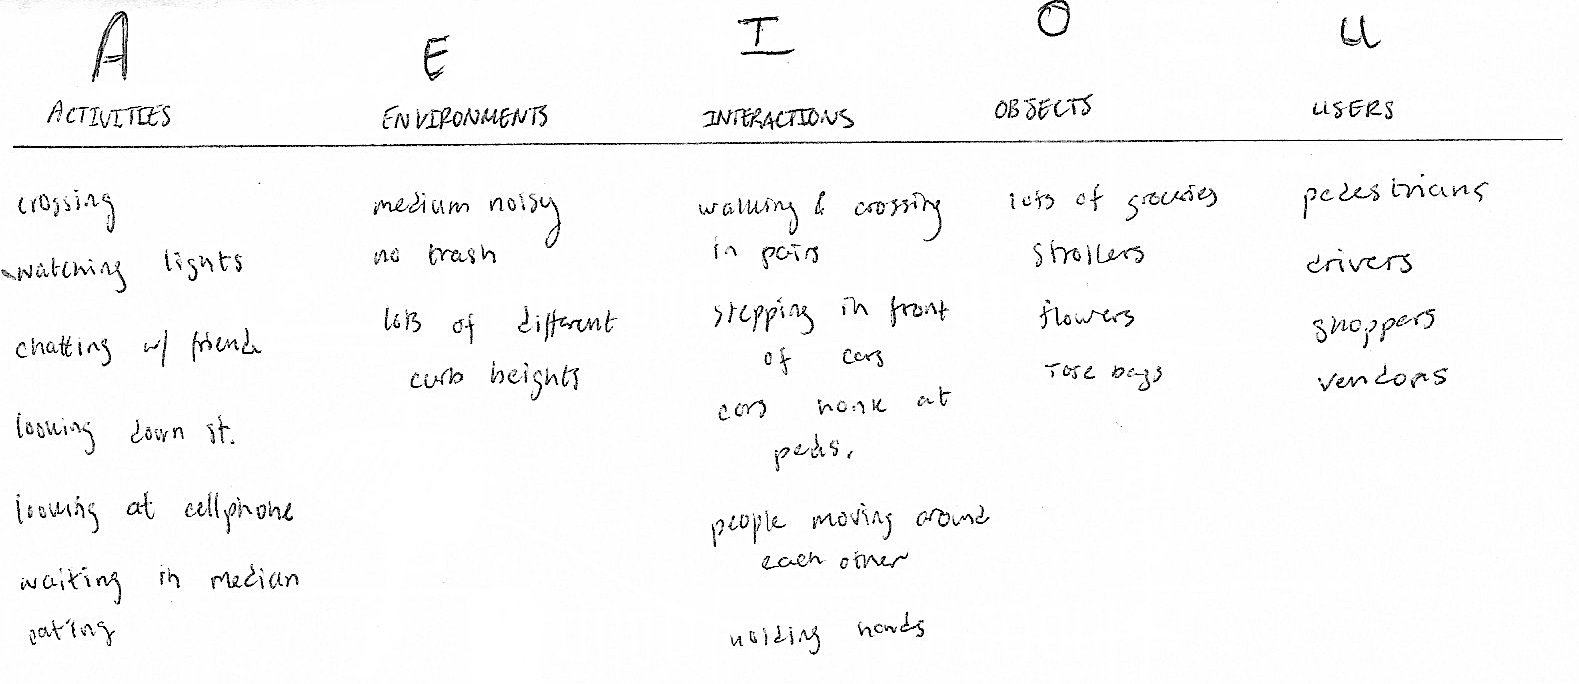
\includegraphics[scale=0.8]{"images/I/ms1_aeiou.png"}\\
\vspace{0.5cm}
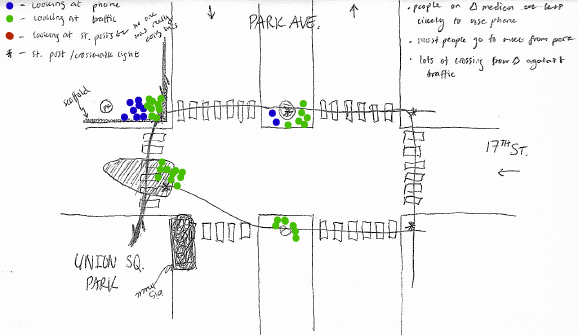
\includegraphics[scale=0.8]{"images/I/ms1_behaviormap.png"}
\caption{AEIOU and Behavior mapping exercise}
\label{fig:behaviormap}
\end{figure}

Behavior mapping at the crosswalk revealed some more interesting data. People waiting at the crosswalk were generally found to be doing one of three things: chatting with a friend, looking at their phone, or looking at traffic. The majority of people waiting at the intersection spent their time looking at traffic. I think this may be due to the fact that this intersection is quite long -- it has a median -- and cars moving down Park Ave. tend to be going pretty fast. It seems like an intersection that requires attention as a pedestrian.  

Since most of the people crossing the street here were travelling to or from the farmer's market and many were with fiends or family, the majority of foot traffic was routed over the small delta in the bike lane (see shaded shape in map) with people clustered in groups. In comparison, few people stopped on the medians in Park Ave. Those that did were generally alone and walking out of sync with the lights and were paying attention to traffic, not their cellphones.


\subsection*{Ideation}

After collecting data, we began to brainstorm about which interactions would be most interesting between strangers crossing the street. The idea of playing a simple game with a strange on the other side of the crosswalk was very appealing, but most required more synchronization and direction than was possible in such a short amount of time (the amount of time spent waiting at the crosswalk).
 
\begin{figure}[ht]
\centering
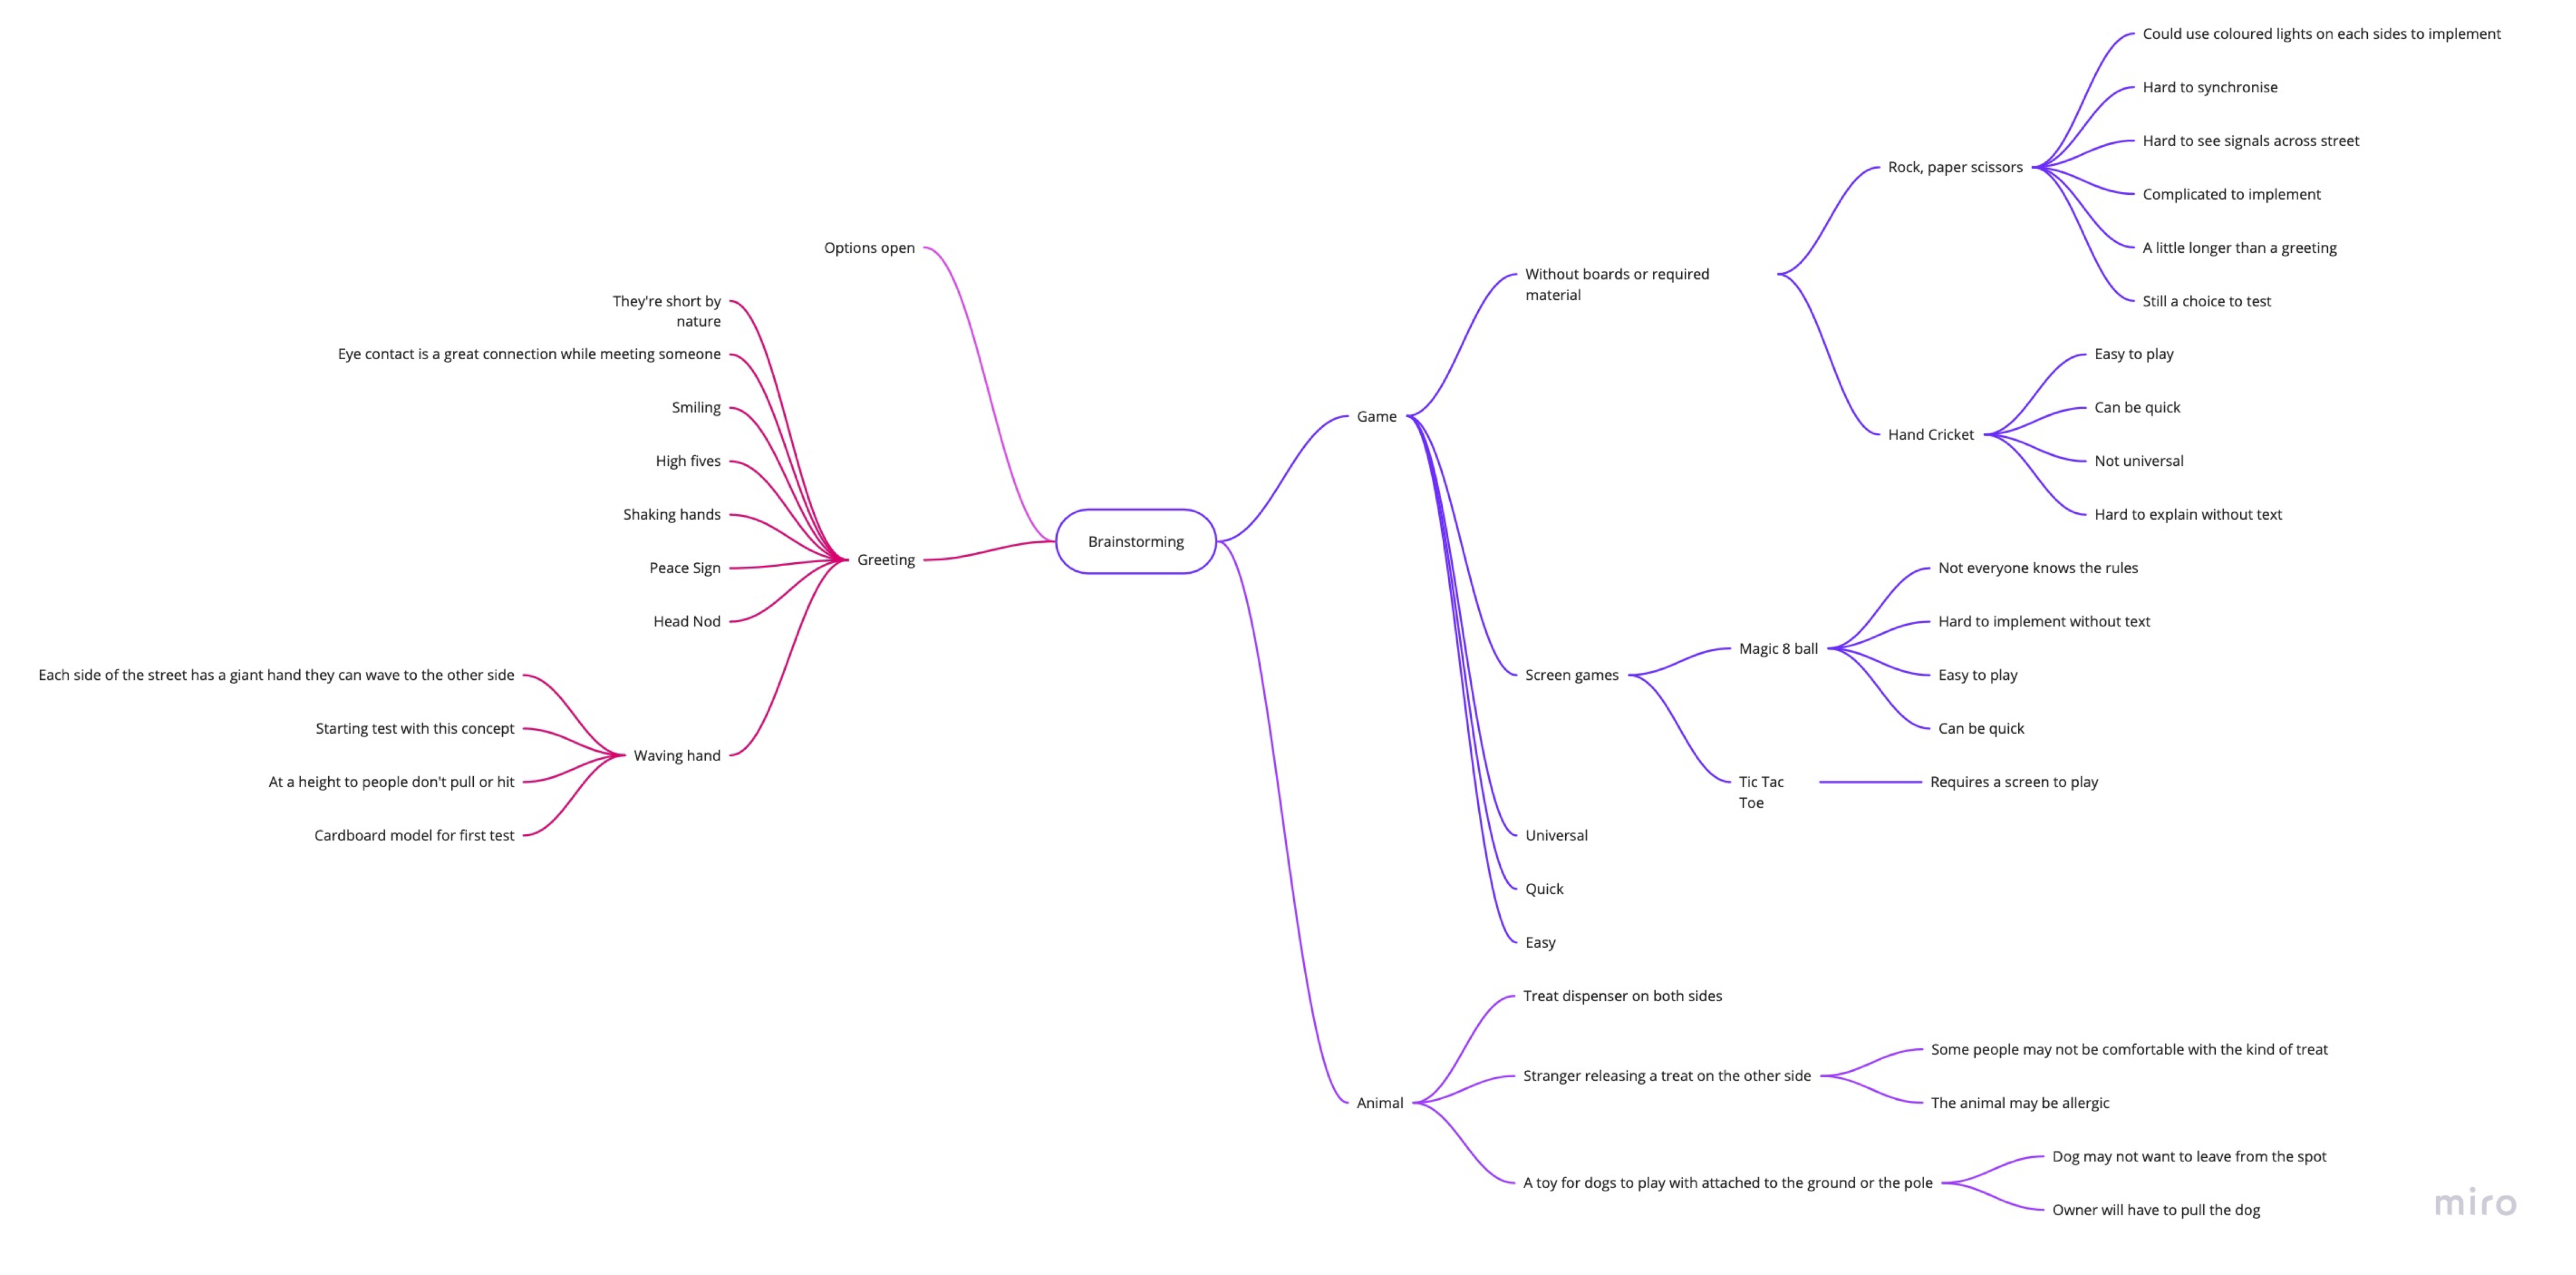
\includegraphics[width=1.4\textwidth, angle=90]{"images/I/ms1_brainstorming.png"}
\caption{Results of brainstorming activity.}
\label{fig:brainstorm}
\end{figure}

After deciding that the ideal interaction would be really quick -- such as a greeting -- we began thinking about fun ways to wave at someone on the other side of the street. The idea of having a giant arm and hand on each side of the street was very appealing and seemed both simple and effective. The below sketch illustrates what a pair of hands / arms would look like on location.
 
\begin{figure}[ht]
\centering
\includegraphics[width=0.8\textwidth]{"images/I/wavemachine_overlay_2.jpg"}
\caption{Sketch of device on location.}
\label{fig:overlay}
\end{figure}

The best part of such a contraption is that it would not necessarily require the use of electronics. Using thin plywood, springs and some clever balancing, we could create the arm mechanism from very basic materials. Below is a sketch of one possible mechanism.
 
\begin{figure}[ht]
\centering
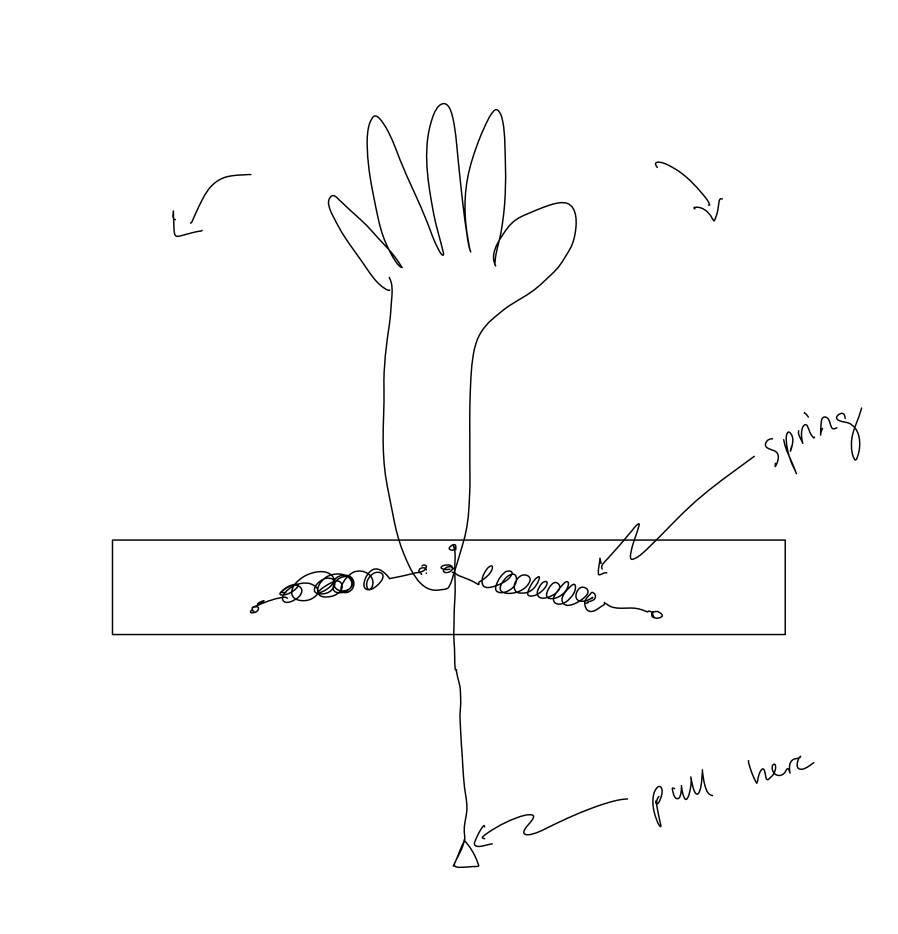
\includegraphics[width=0.8\textwidth]{"images/I/wavemachine_sketch.png"}
\caption{Possible mechanical design of device.}
\label{fig:sketch}
\end{figure}

\clearpage
\section*{PART II - Iteration}
\subsection*{initial prototypes}

The initial prototype was extremely quick. It successfully proved that the basic mechanism did, in fact work. \href{https://drive.google.com/file/d/1A-JF5d3mOUxOp_nL0GExQ2gzeuzpgY3x/view?usp=sharing}{Link to video of initial prototype.}

\begin{figure}[ht!]
\centering
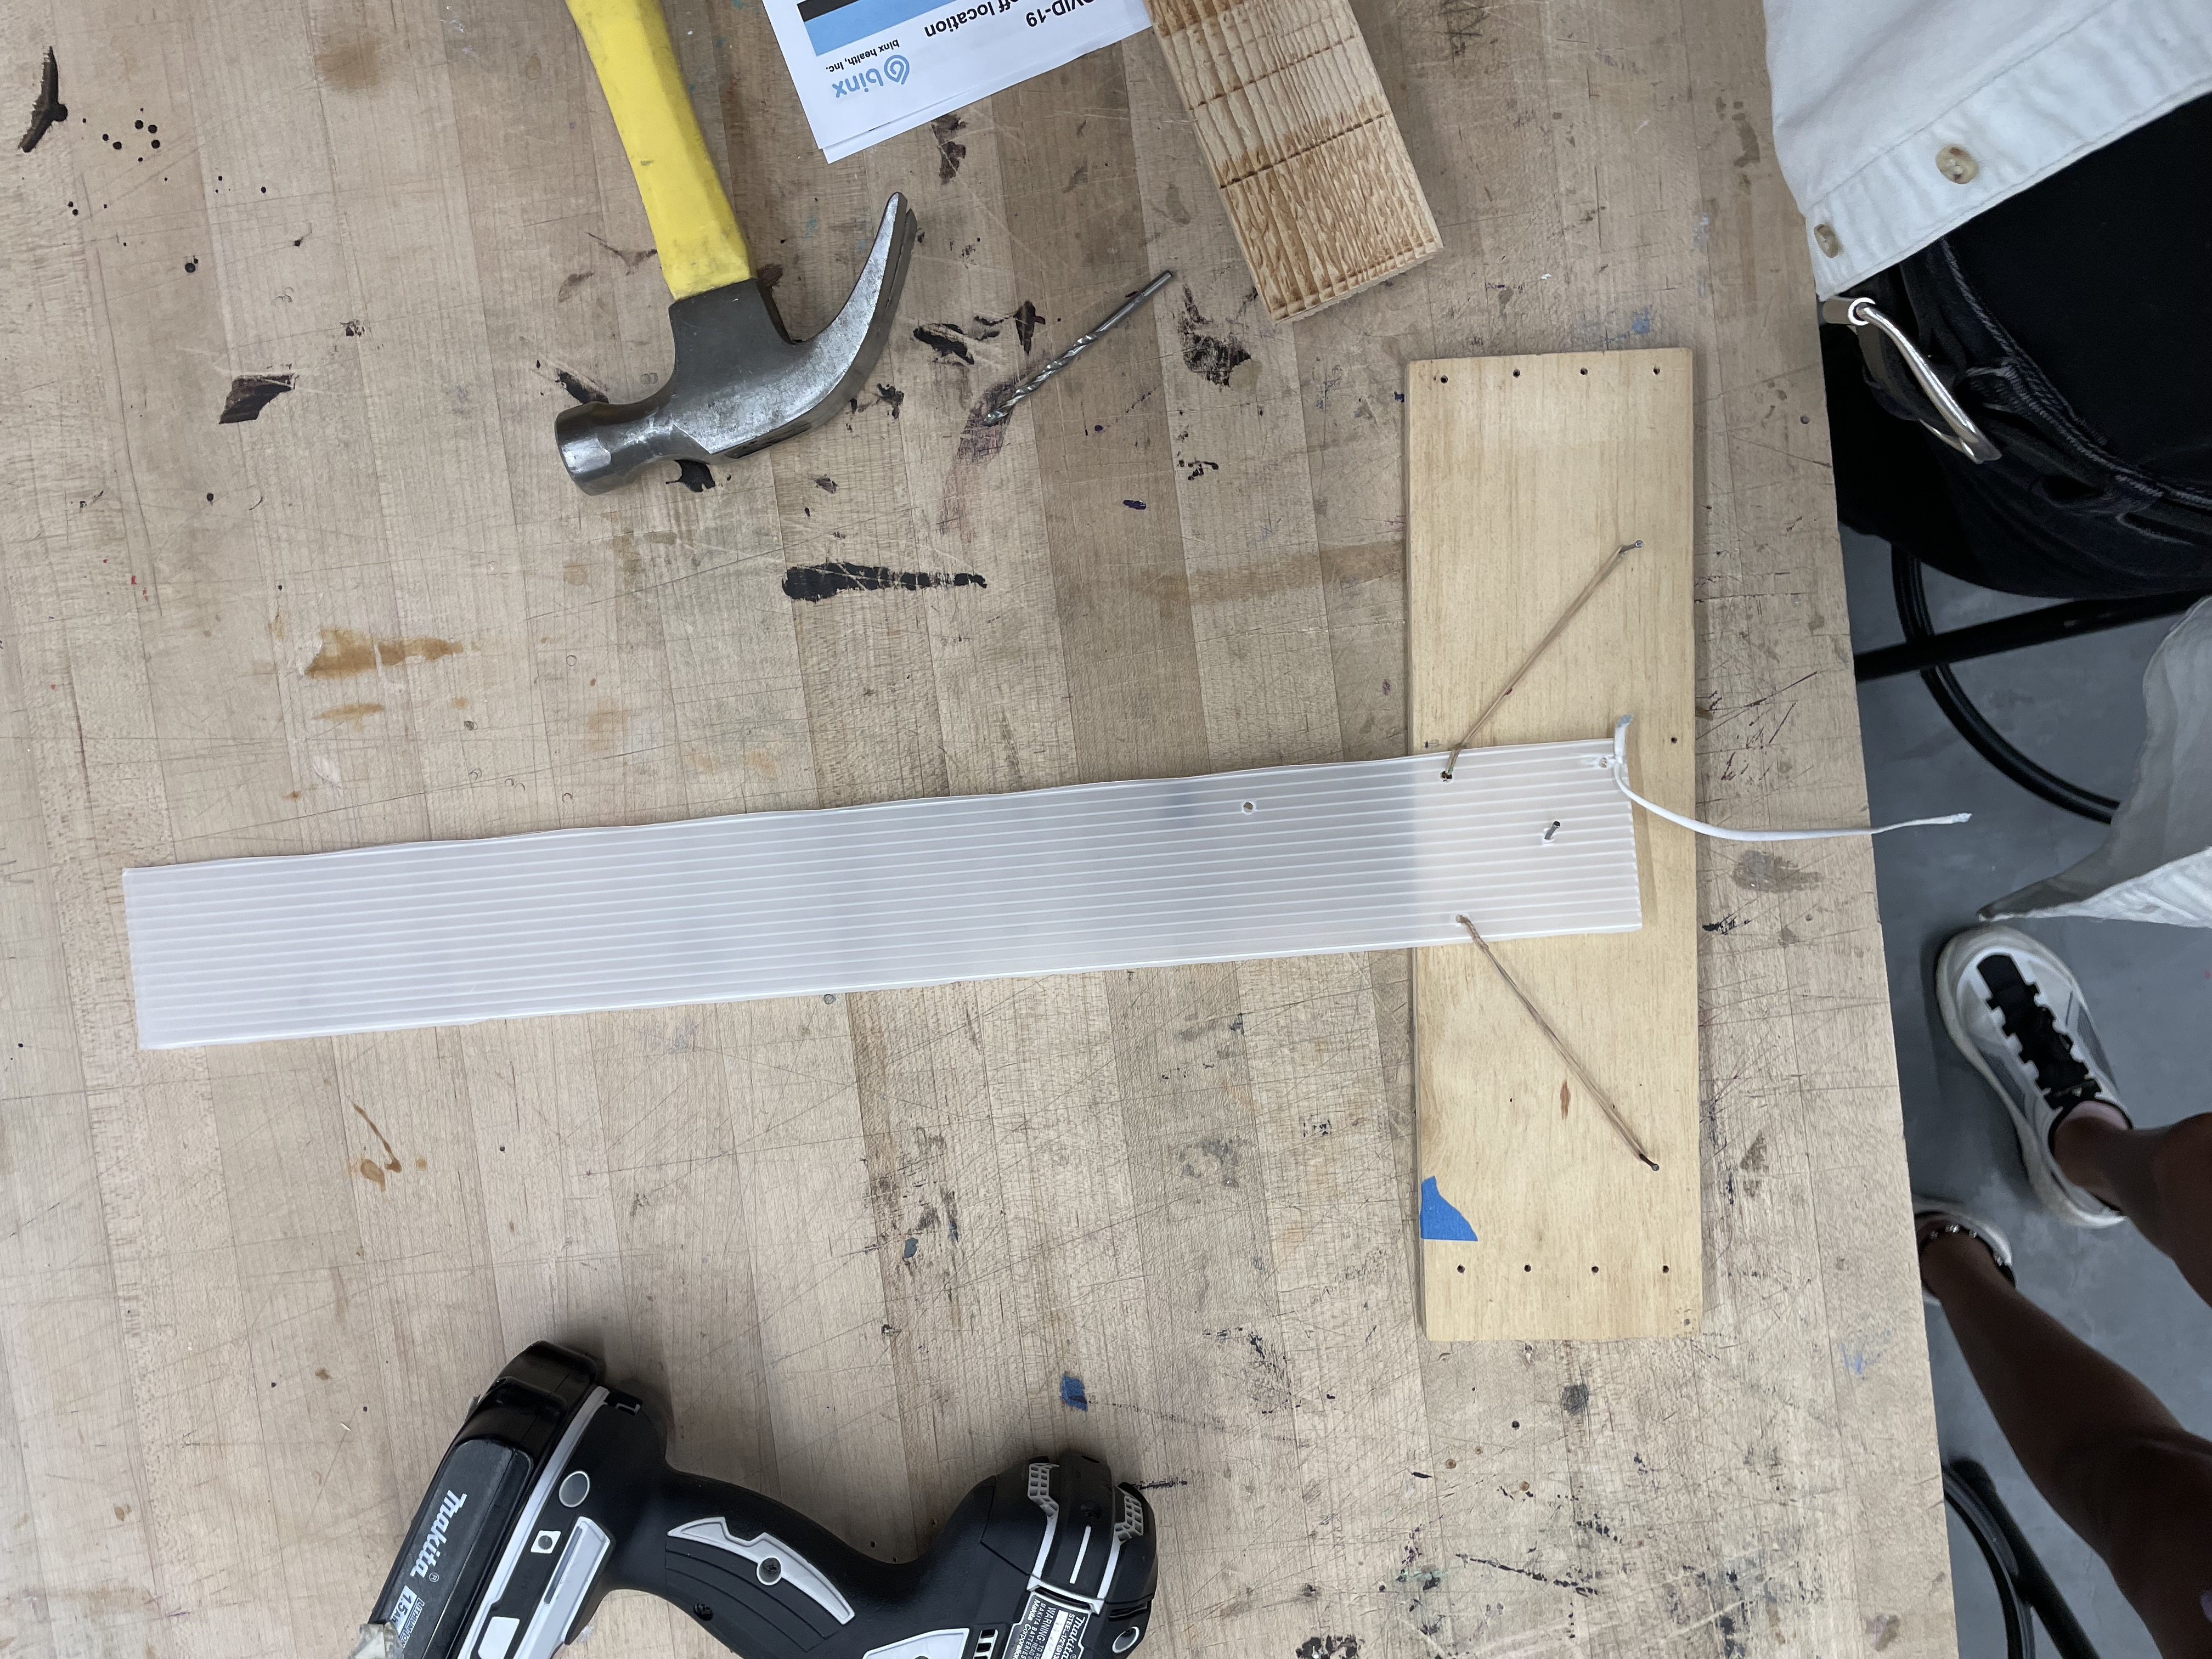
\includegraphics[width=0.8\textwidth, angle=-90]{"images/II/prototype_1.JPG"}
\caption{Initial prototype.}
\end{figure}

The initial prototype required improvement in four areas; a more solid connection between the arm and the base, a way for the base to be connected to a street post securely, improved elastic, and an eye catching handle.

Using a bolt and some washers the arm and the base were connected in a way that allowed the arm to swing freely without twisting. Next, in order to mount the wave machine, we found some large zip ties and drilled holes in the base to thread the zip ties through. During this process we discovered that making the mechanism one-sided decreased the complexity of the device and made it easier to mount the base. By restricting the movement to be one-sided we also decreased the chance of the arm becoming stuck in either direction. Despite the reduction in range, it was still quite satisfying to use the mechanism. As we played with the movement of the arm, the easiest elastics on hand were hair-ties. By trying a couple different sizes we honed in on the best tension for the weight of the arm. Finally, we cut the end off of an aluminum mop and colored it bright red with a sharpie in the hope that this would grab someone's attention. \href{https://drive.google.com/file/d/10h-Otp0xxu8sbUBII9ftw7f-XZoaok2H/view?usp=sharing}{Link to video of second prototype.}


\begin{figure}[ht!]
\centering
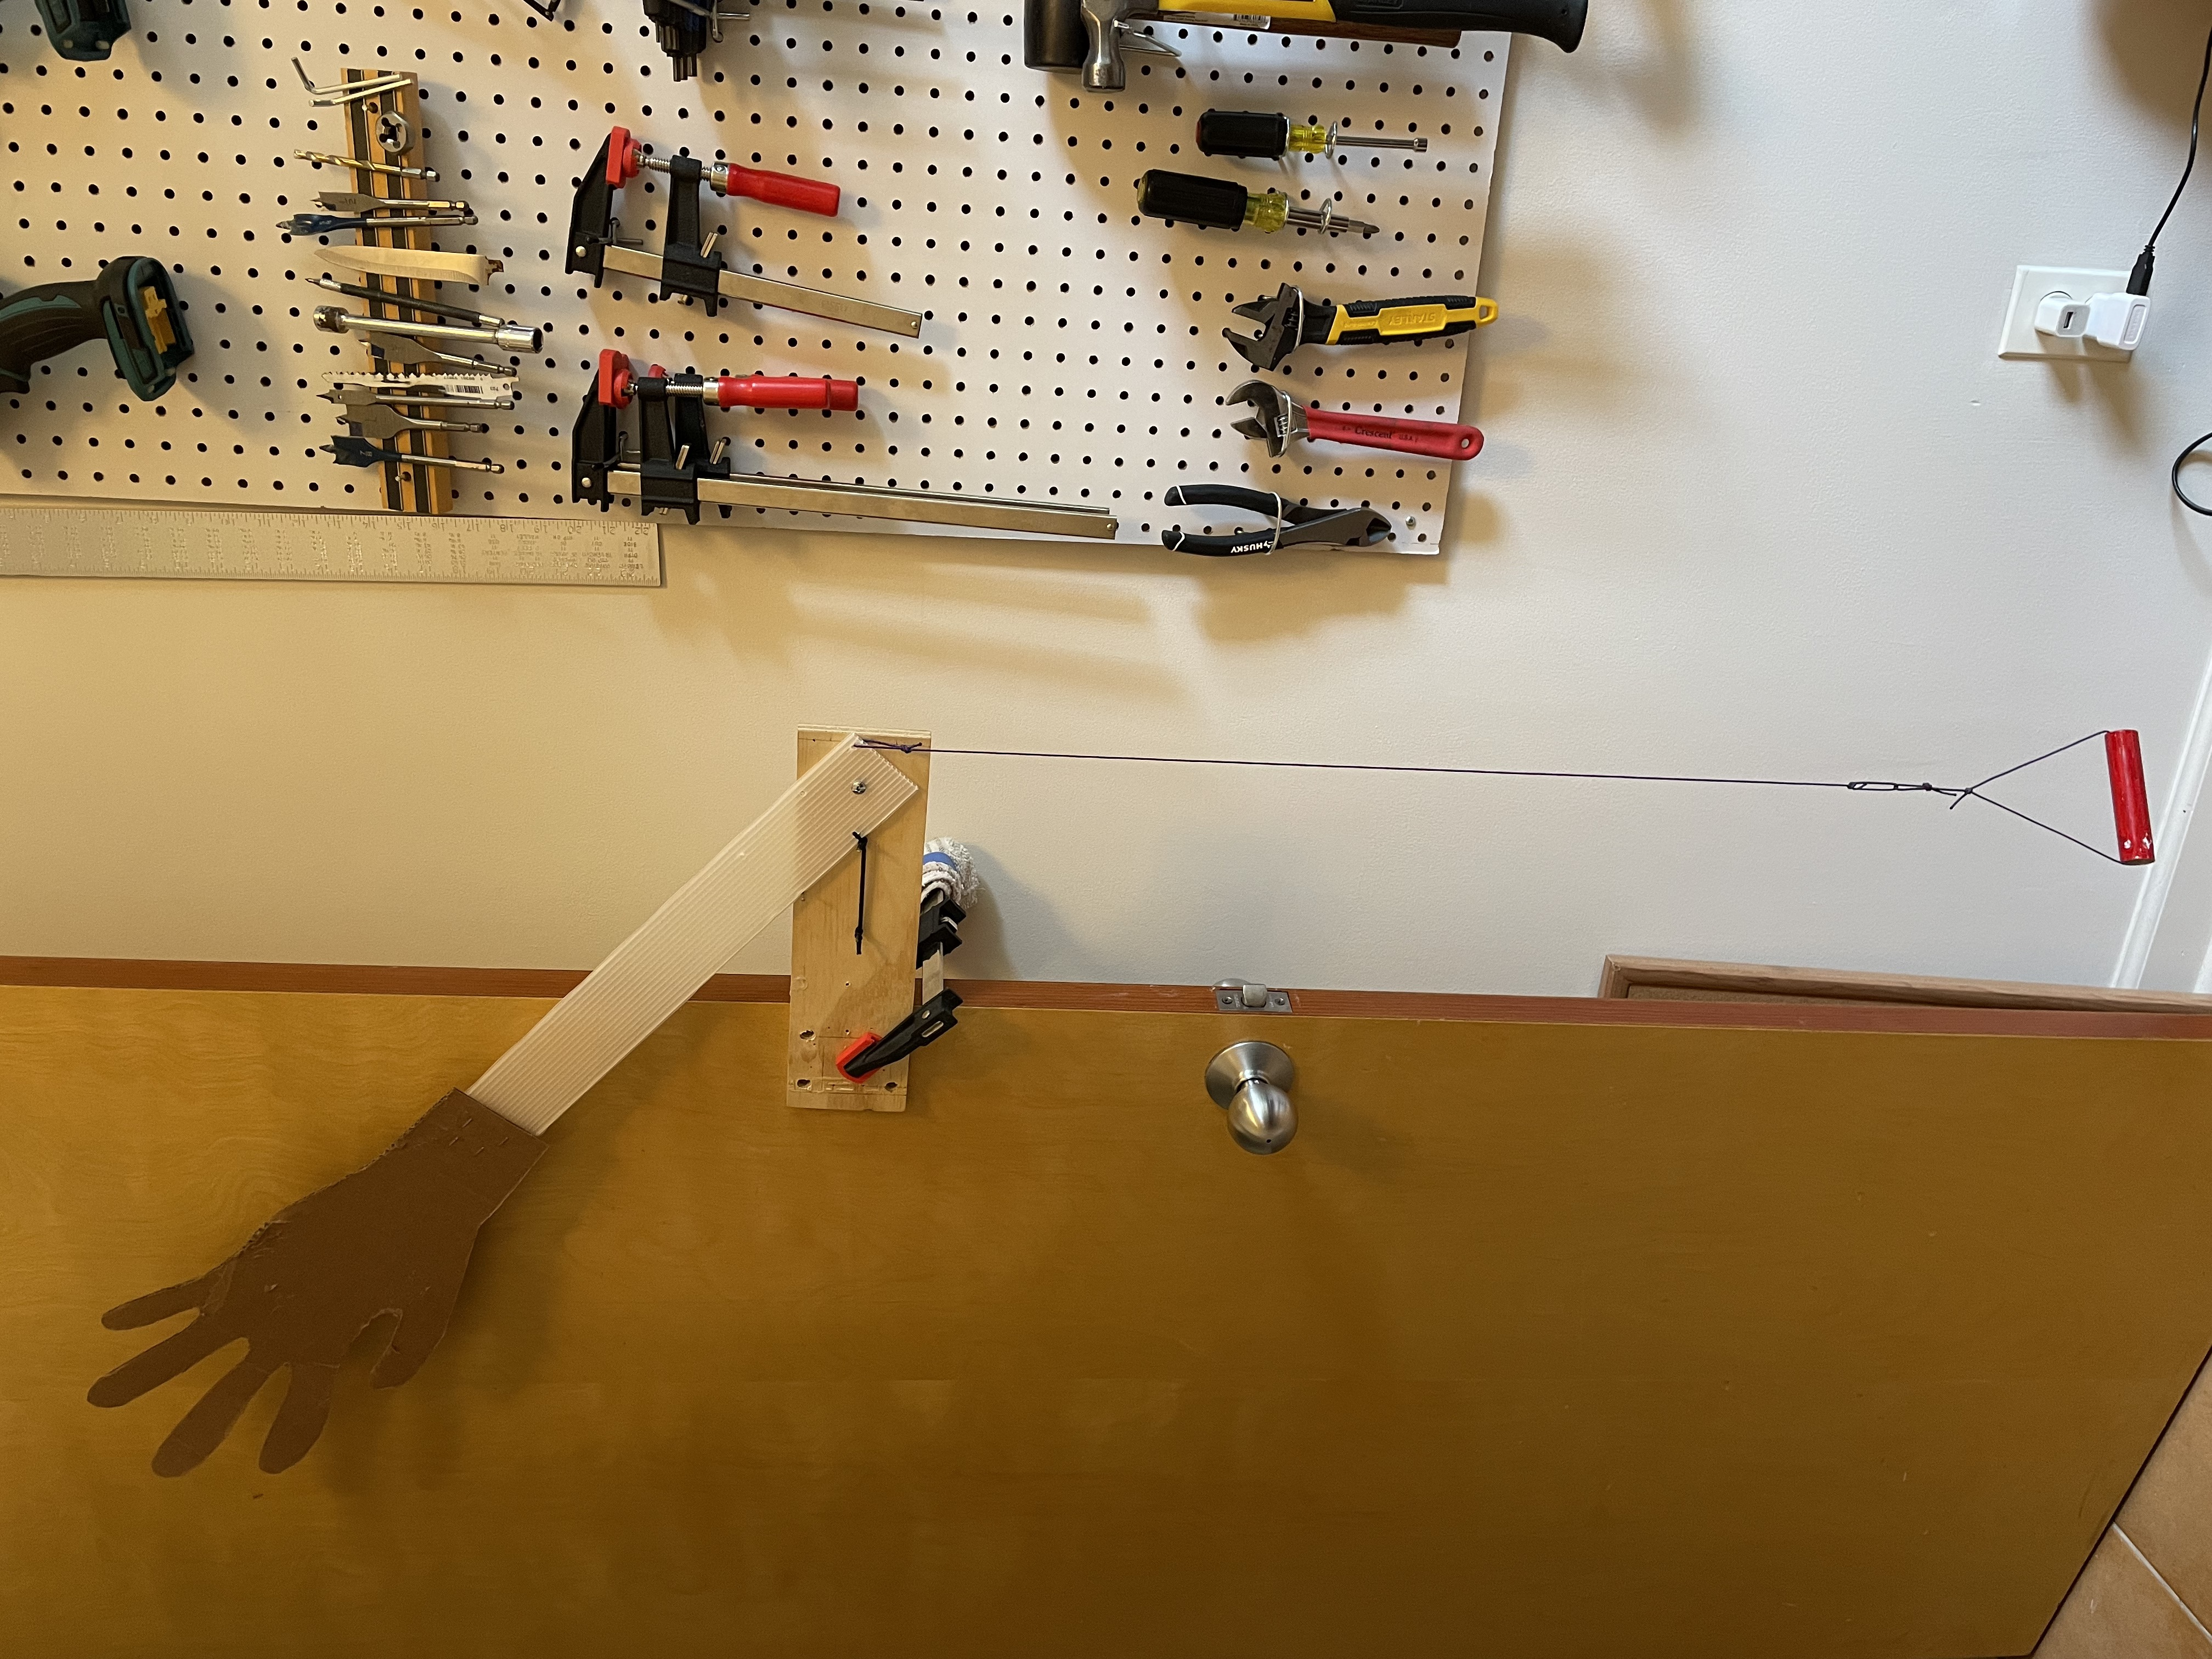
\includegraphics[width=0.8\textwidth, angle=-90]{"images/II/prototype_2.JPG"}
\caption{Initial prototype.}
\end{figure}

\subsection*{testing results}

Due to time constraints, we chose to test the wave machine close to home instead of at the proposed site. Installation went well; it was easy to attach the base securely to the street post and then adjust it to be out of the way of the crosswalk signals. Pulling the handle was satisfying and the motion of the mechanism was smooth and effective. It was fairly visible from across the street when the arm was waving. \href{https://drive.google.com/file/d/1Gzw53p0xpSqZ-RktlmBlWZ7QyR_WPB5E/view?usp=sharing}{Link to video of installed protptype.}

\begin{figure}[ht!]
\centering
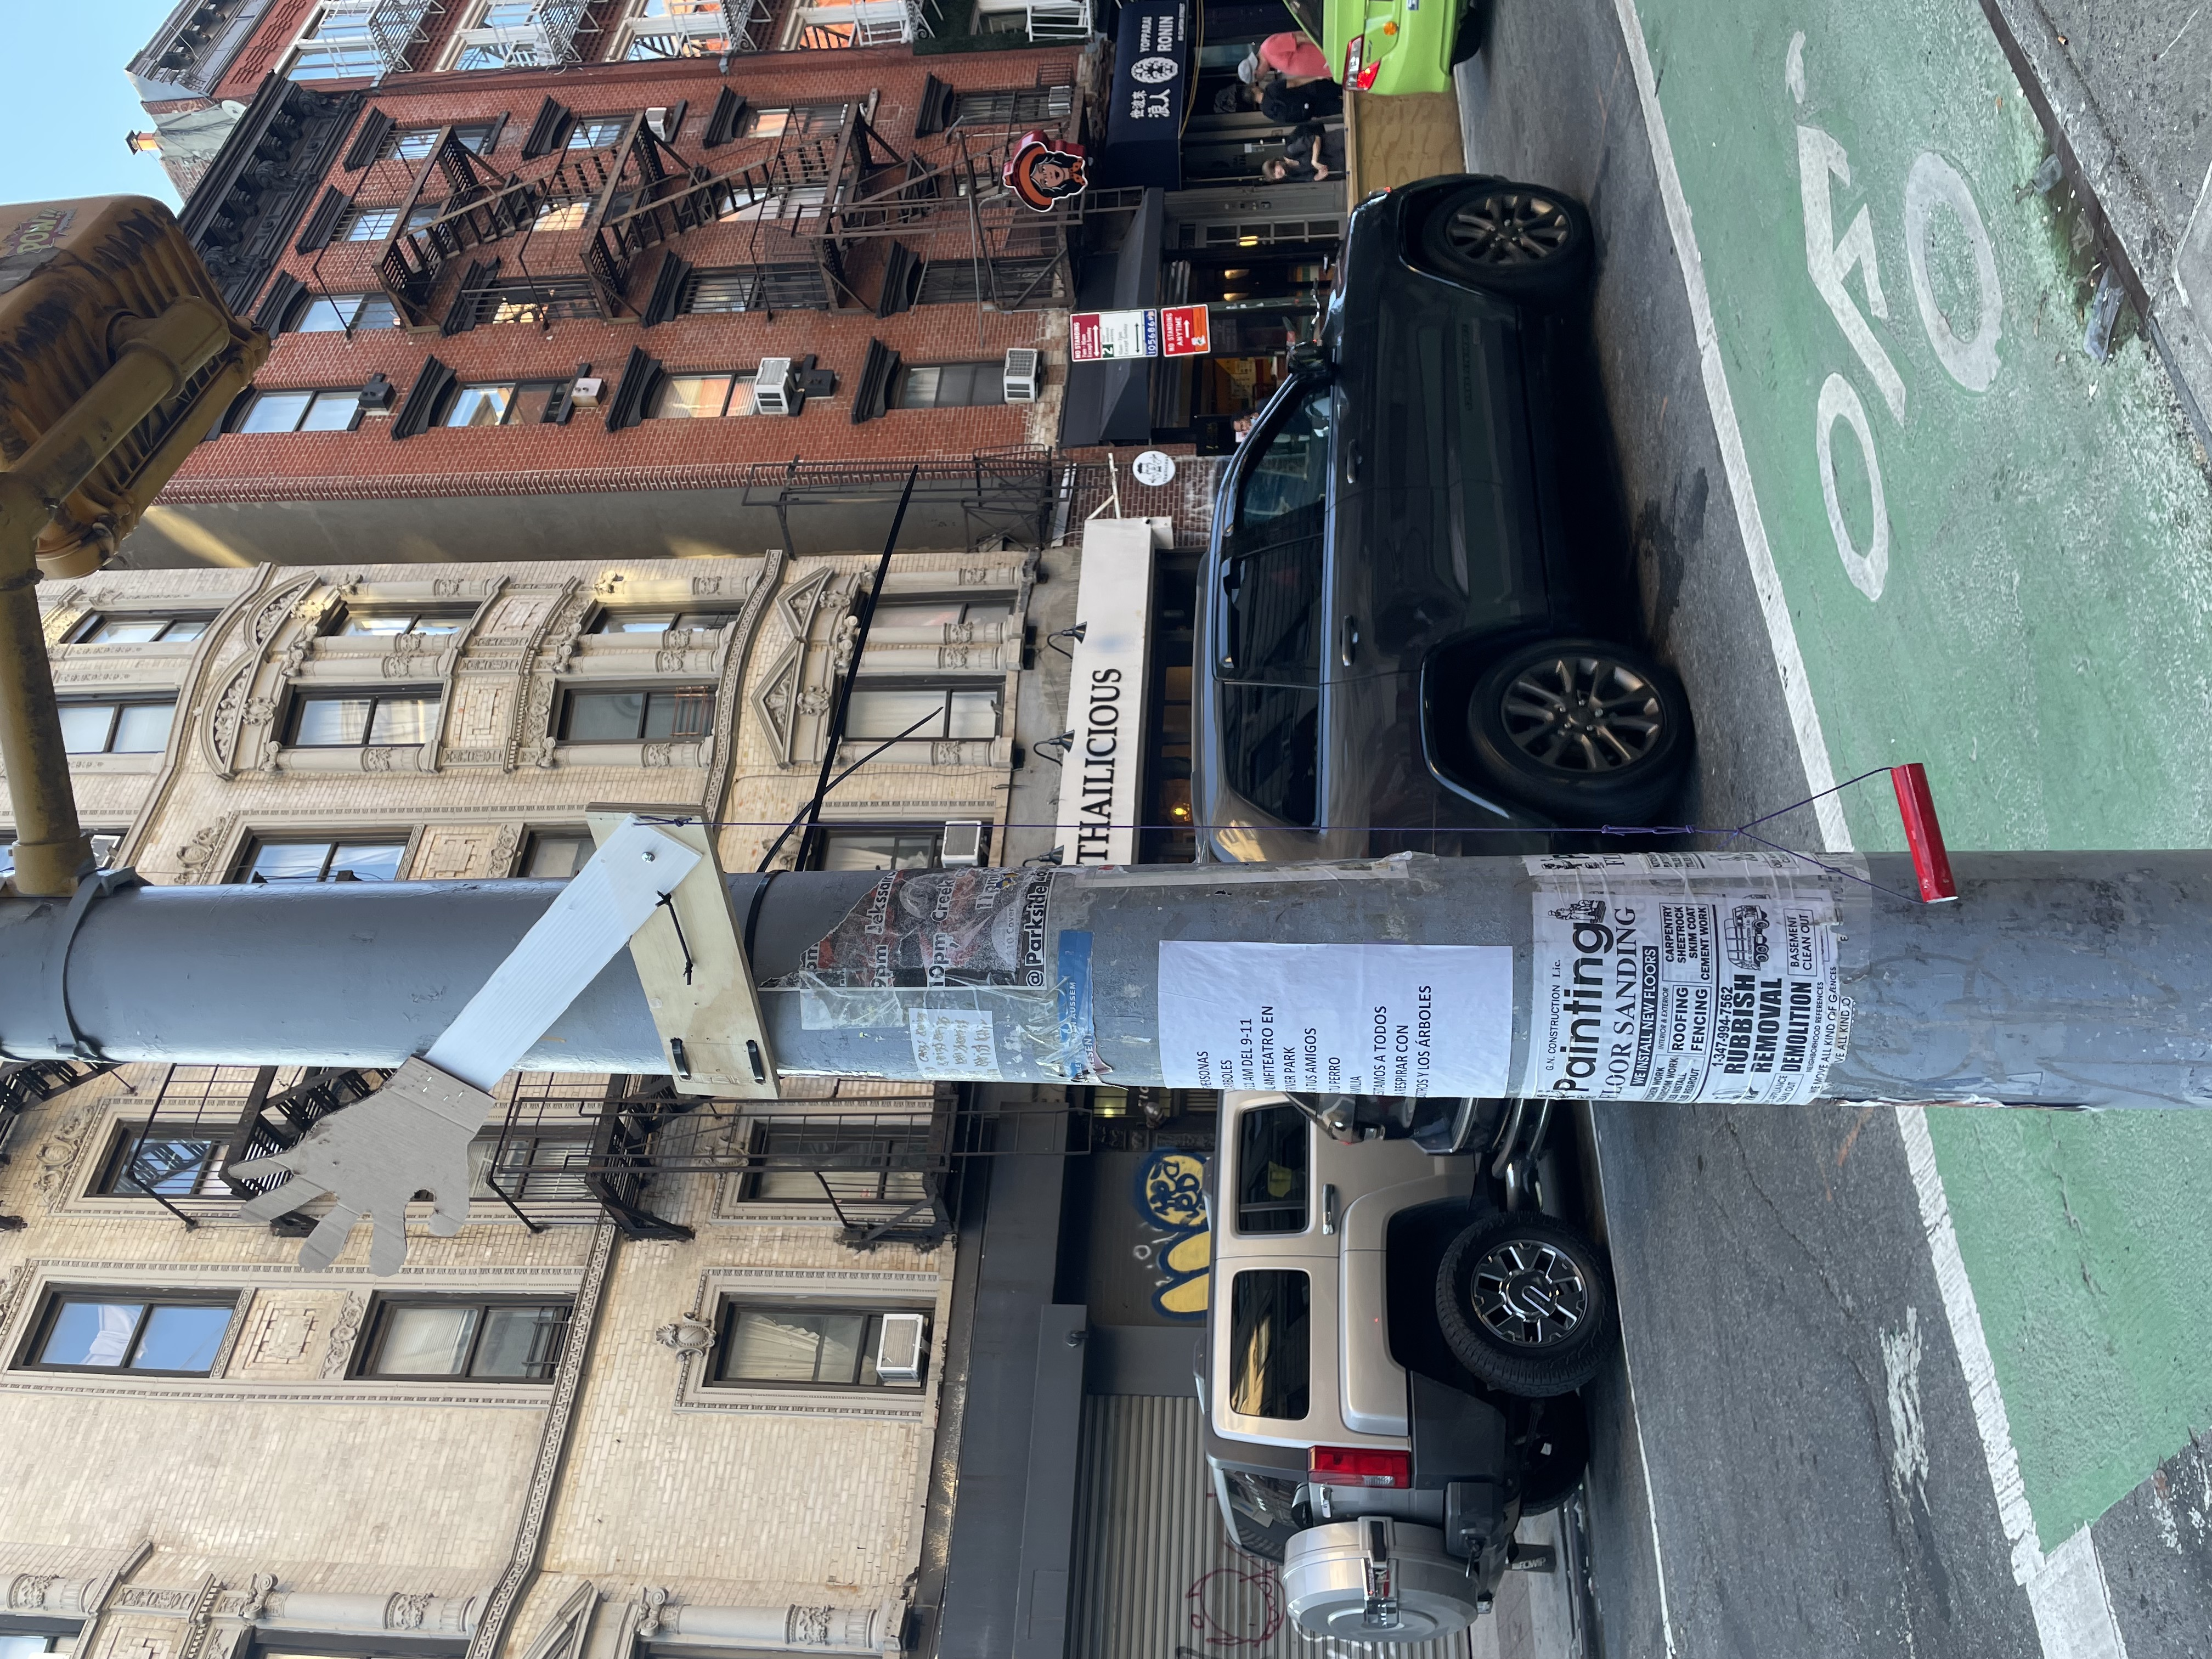
\includegraphics[width=0.5\textwidth, angle=-90]{"images/II/install_closeup.JPG"}
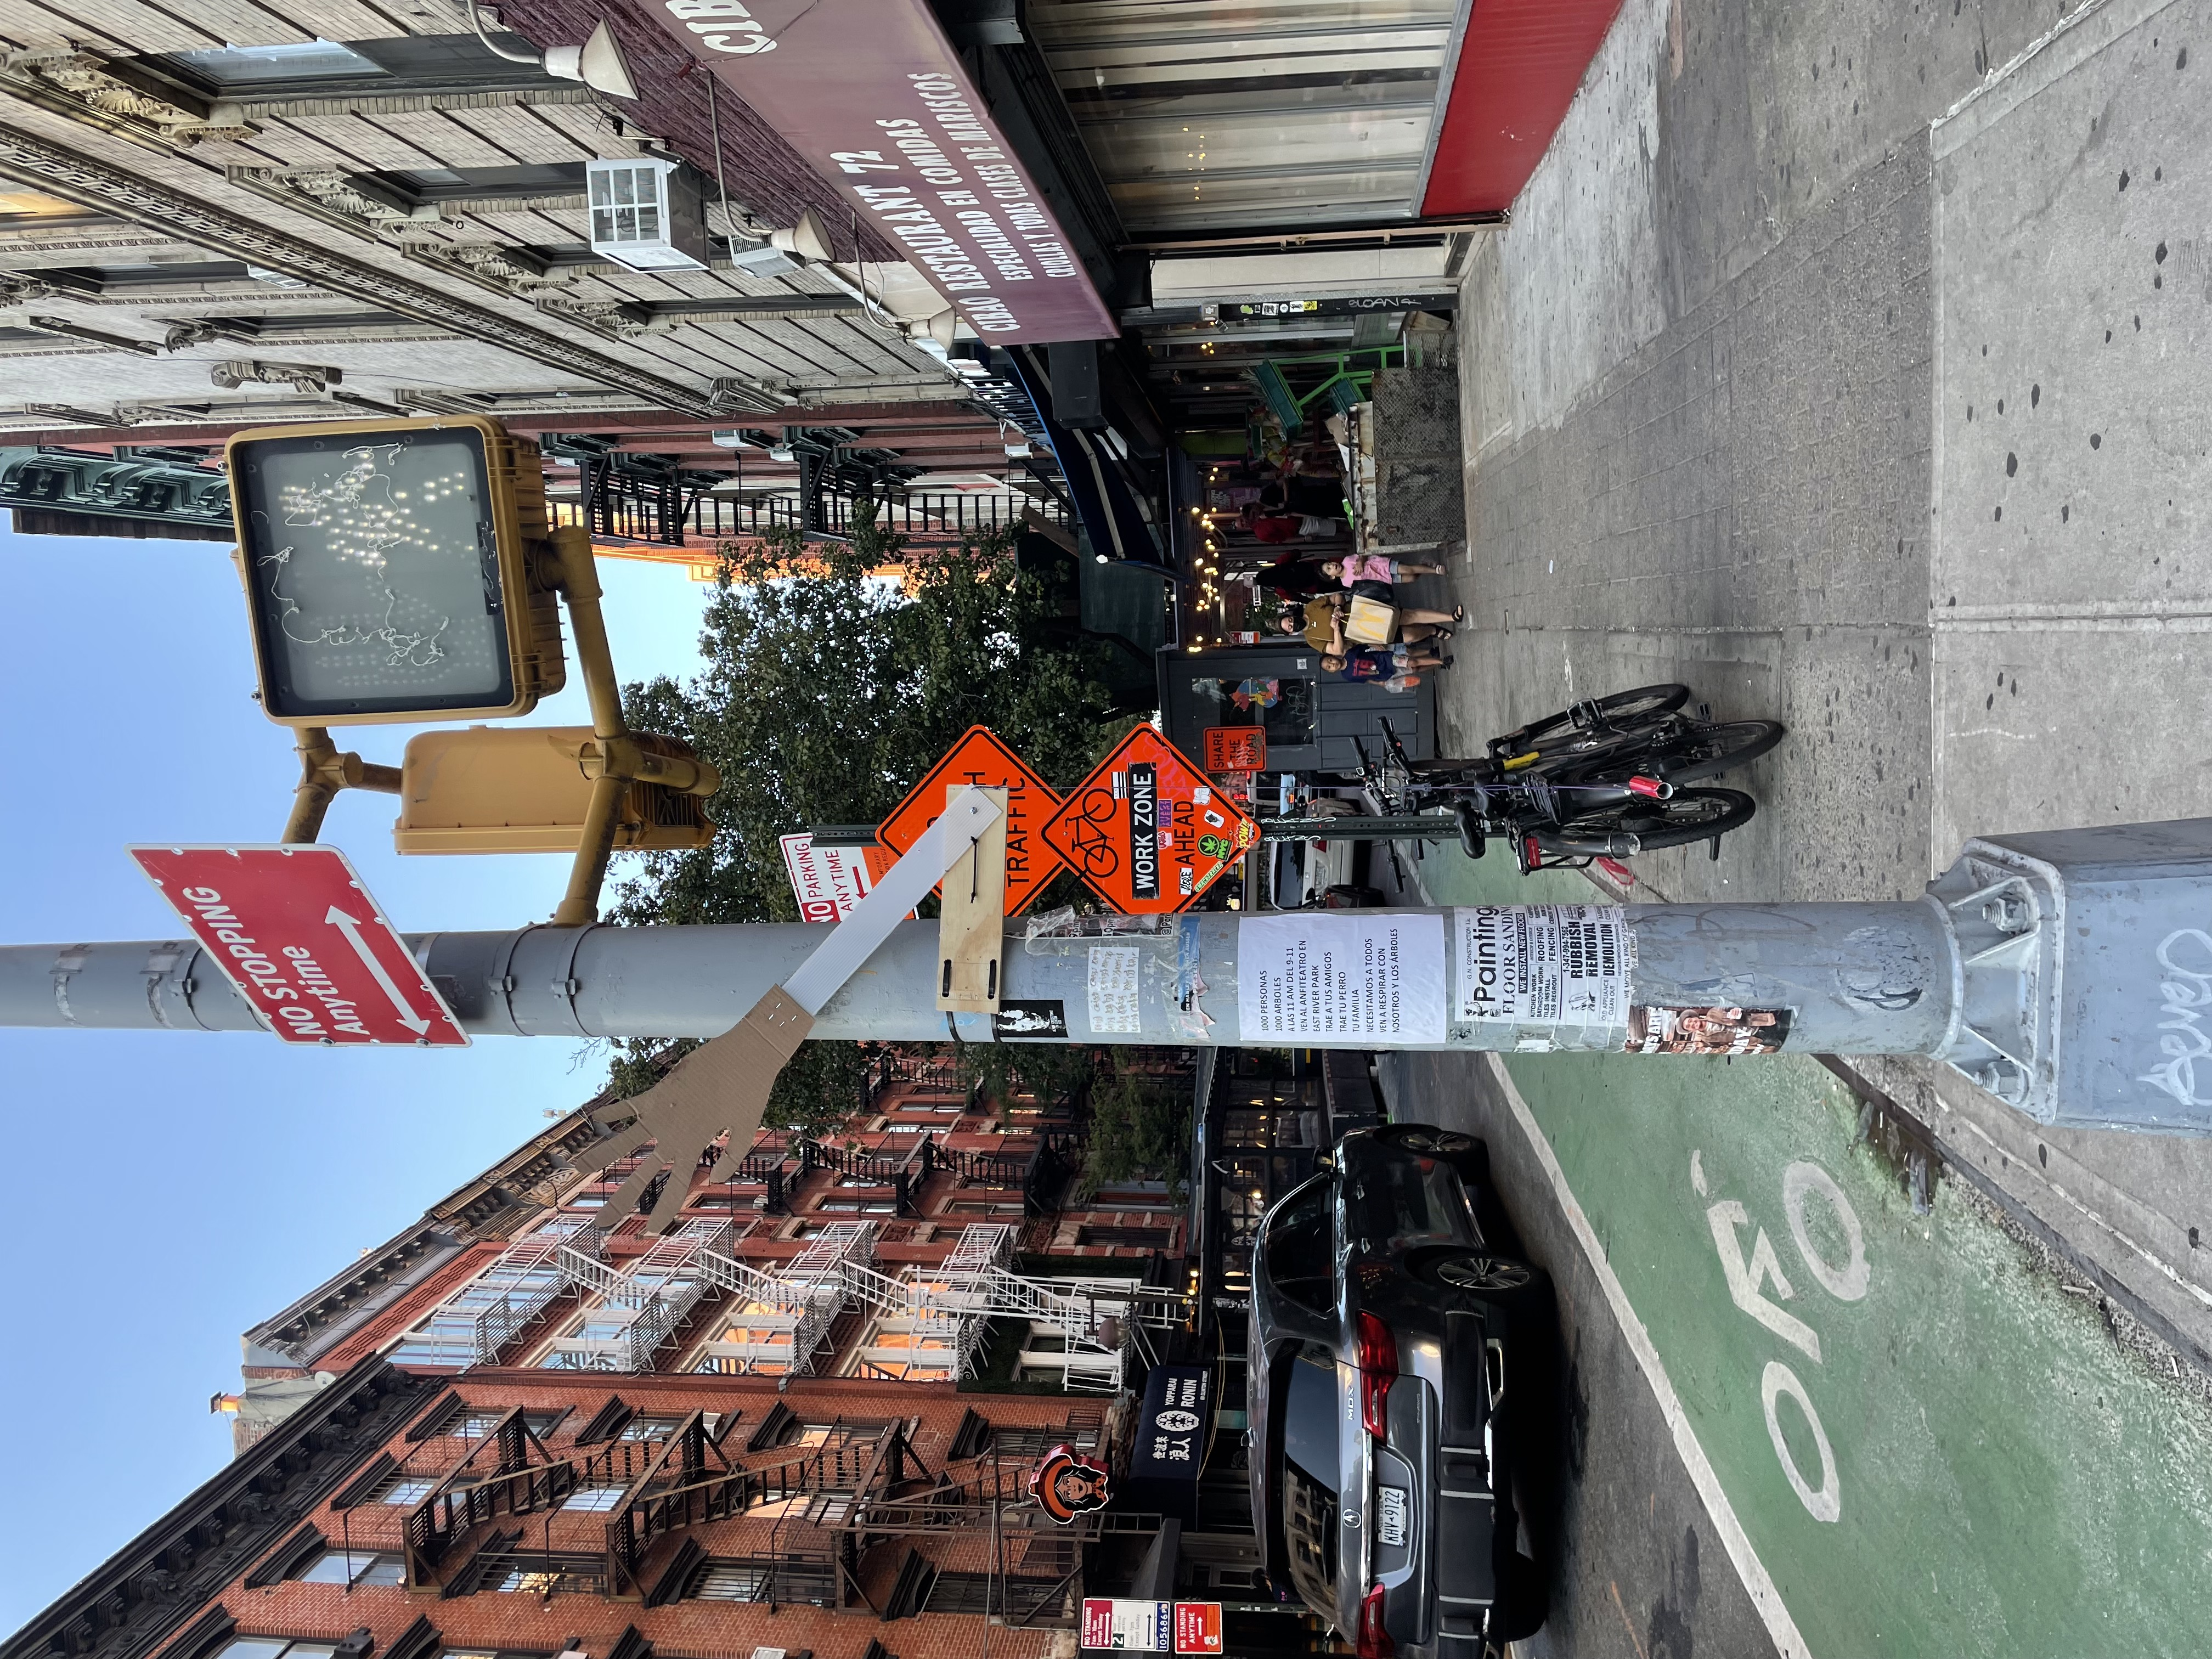
\includegraphics[width=0.5\textwidth, angle=-90]{"images/II/install_closeup_2.JPG"}
\caption{Installed mechanism.}
\end{figure}

\begin{figure}[ht!]
\centering
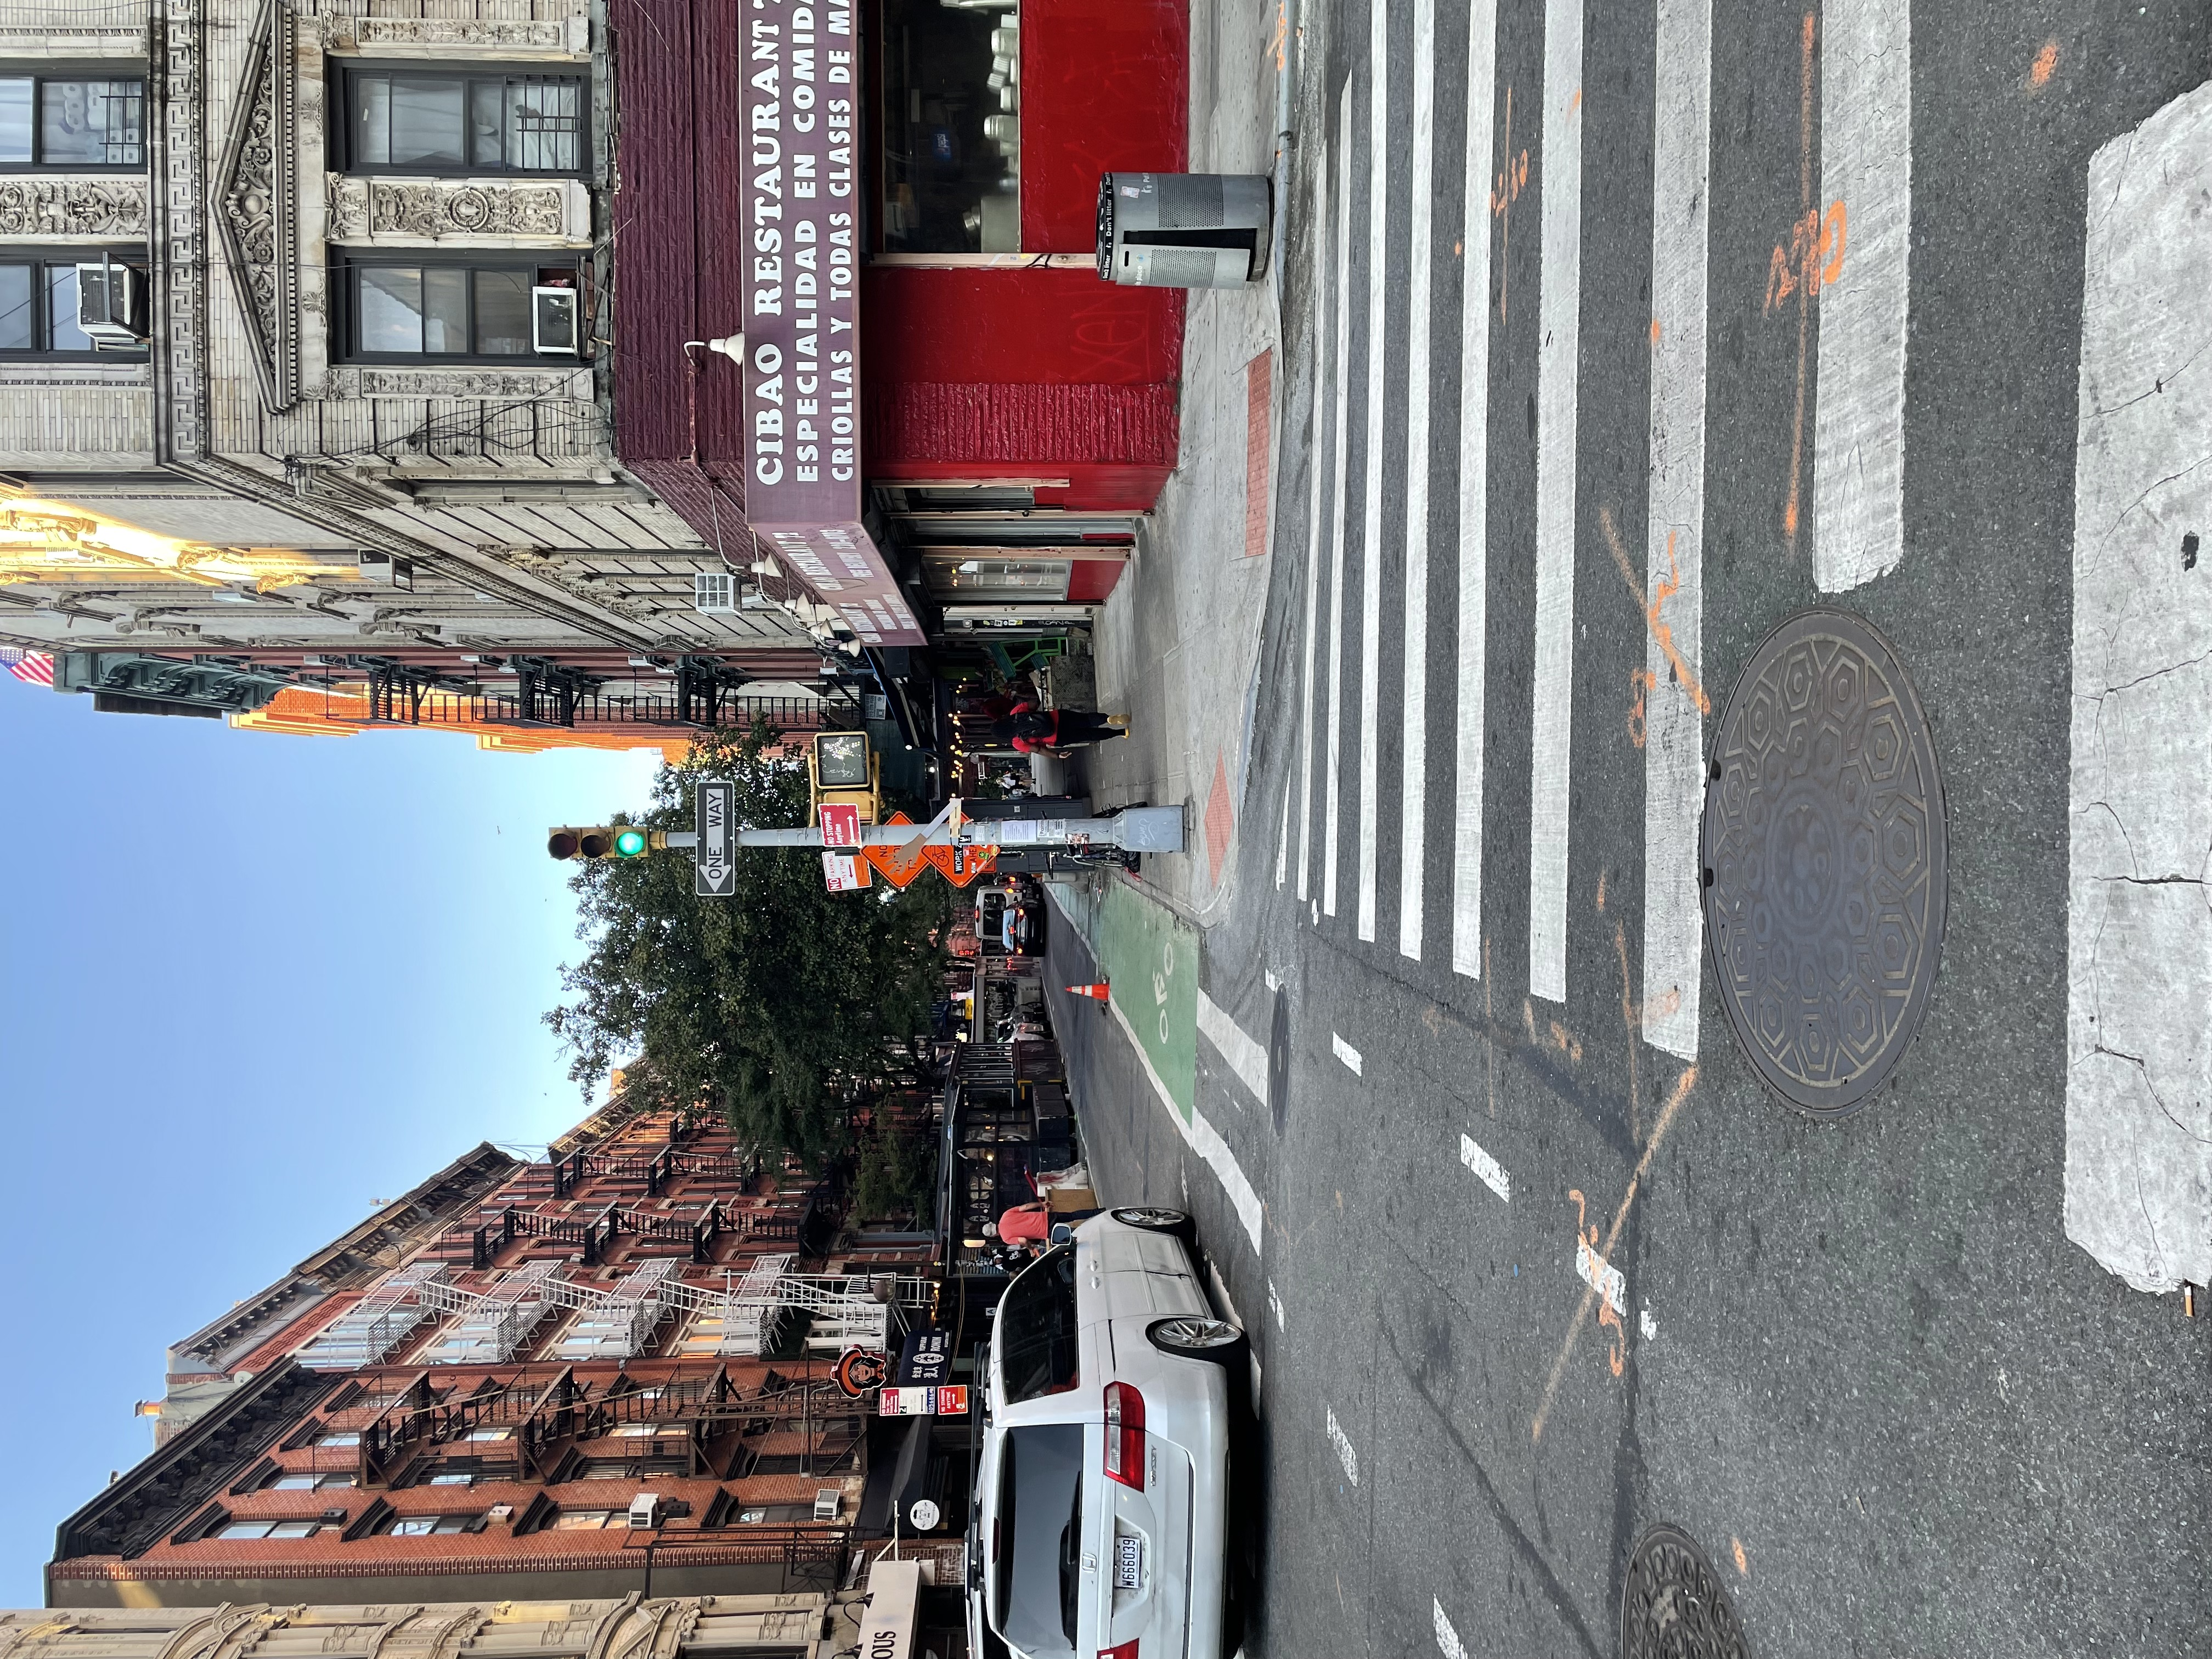
\includegraphics[width=0.8\textwidth, angle=-90]{"images/II/install_far.JPG"}
\caption{Installed mechanism.}
\end{figure}

Unfortunately, while the chosen time and location yielded a high degree of foot traffic, few noticed the wave machine. A few people looked at it, but no one pulled the handle. One person waved back at us while we were using the machine and a few others smiled. Other than that, the initial testing was successful for mechanical refinement, but not so much for user feedback.

\subsection*{next steps}

It was clear after initial testing that the wave machine needed to be more noticeable and the chosen location needed to be more heavily trafficked by individuals out looking for fun. In addition to making the mechanism robust enough to stand up to real use, three modifications were decided upon: improved location, more visible arm, more alluring handle.

We happened to witness a particular crosswalk that was very crowded on both sides late at night. Nearly all of the people on both sides of the street were going to or from bars and were already pretty intoxicated. Many people near the crosswalk were waiting in line to enter various bars. Other than trying to get to the line, none of these people were in a particular rush. 

\begin{figure}[ht!]
\centering
\includegraphics[width=0.3\textwidth]{"images/II/elwire.jpg"}
\caption{Electroluminescent wire.}
\end{figure}

\begin{figure}[ht!]
\centering
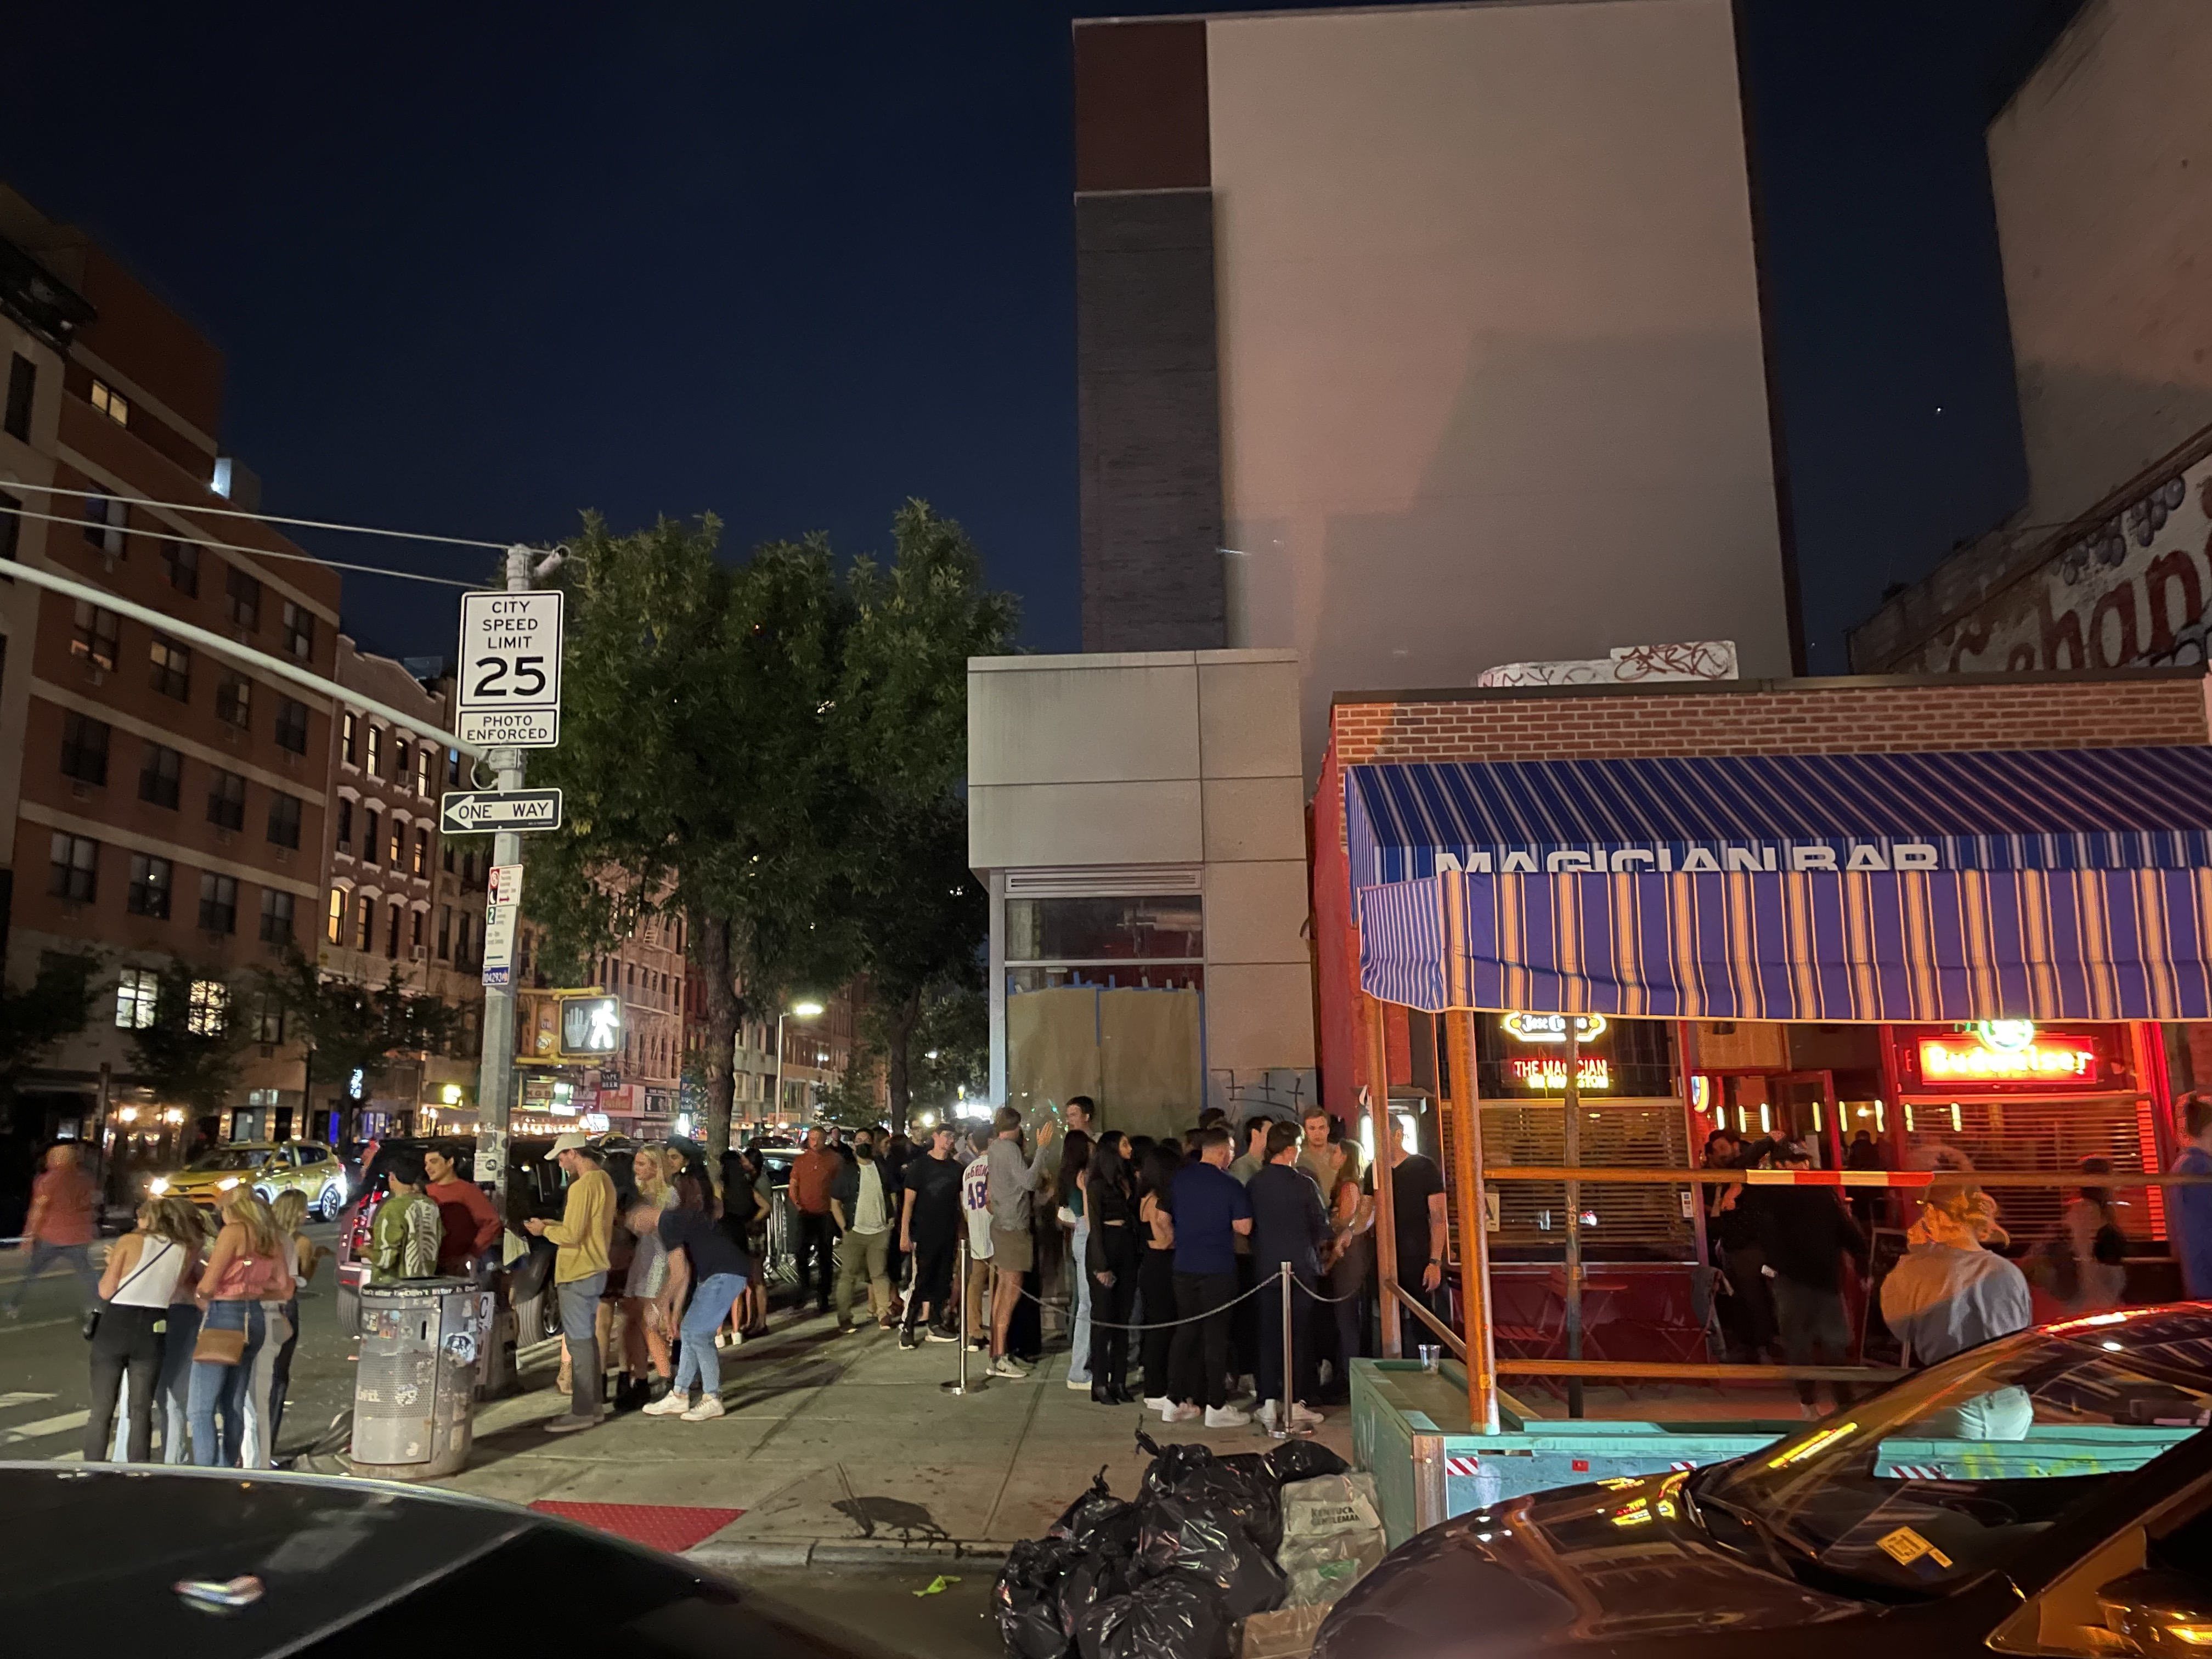
\includegraphics[width=0.8\textwidth]{"images/II/essex_magicianbar.JPG"}
\\
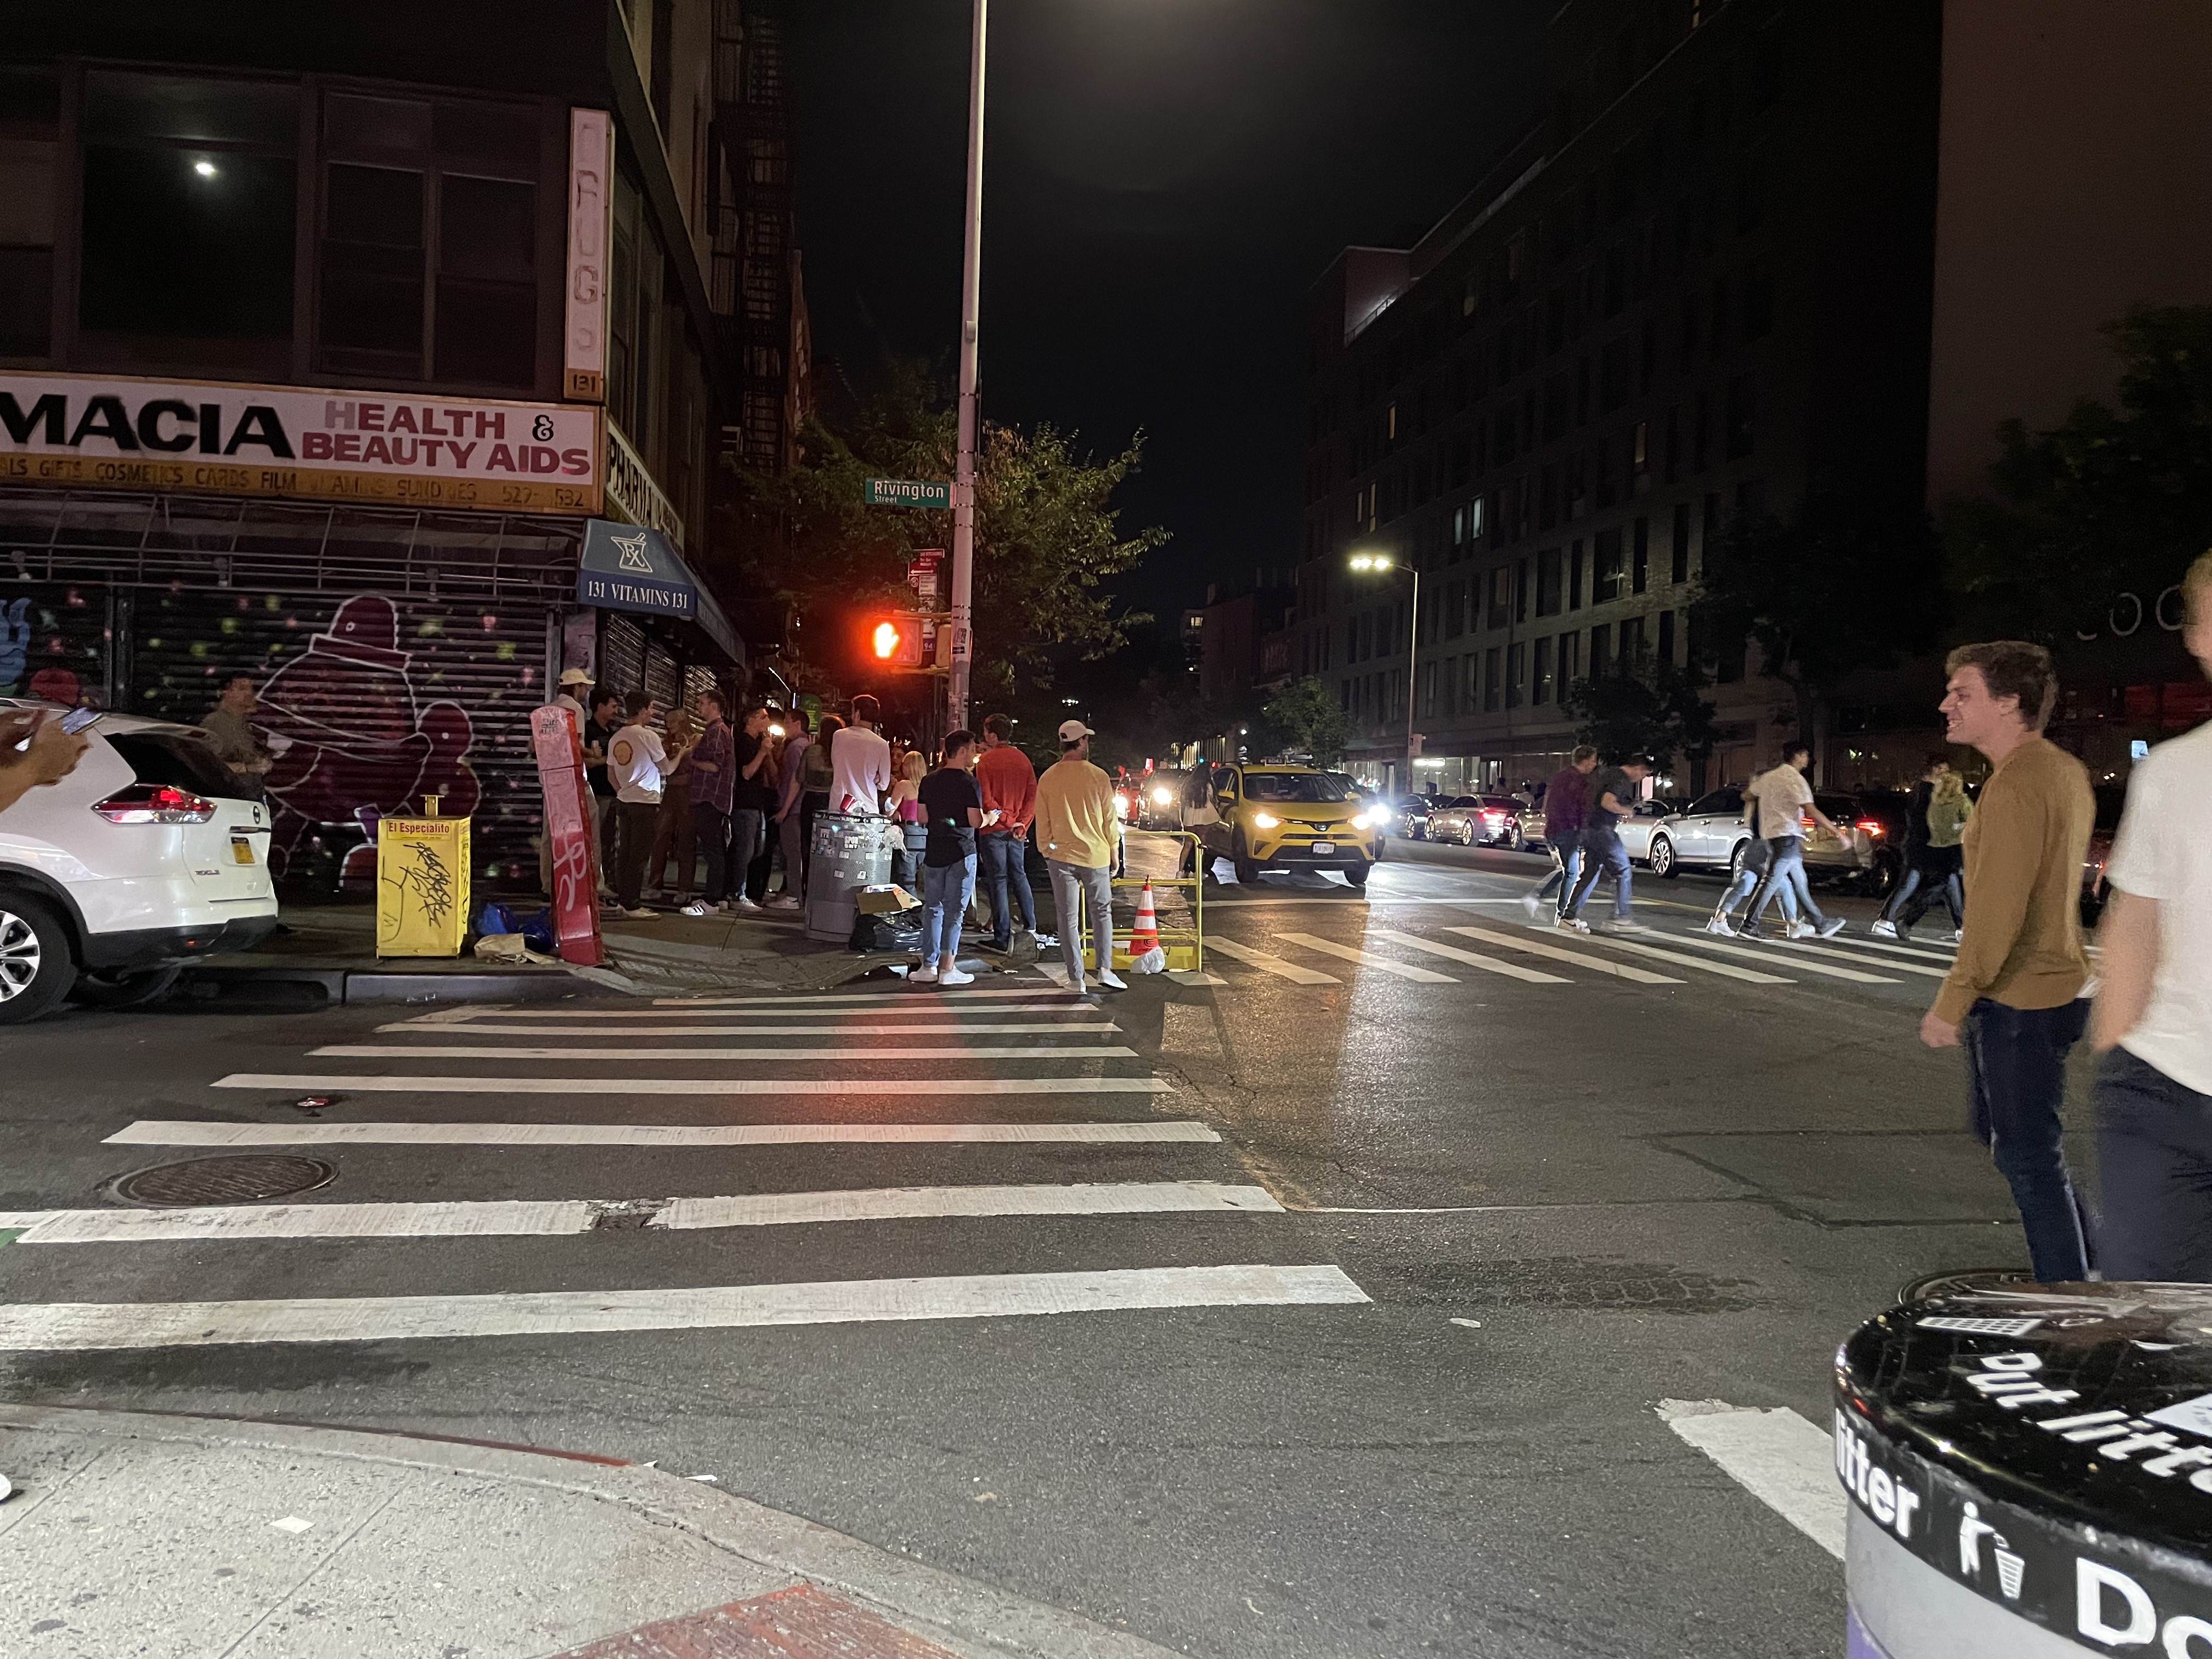
\includegraphics[width=0.8\textwidth]{"images/II/essex_opposite.JPG"}
\caption{Nightlife on both sides of proposed crosswalk.}
\end{figure}


Using electroluminescent (EL) wire we planned to increase the visibility of the arm. The EL wire would be placed around the outline of the arm and hand and could be set to be constantly on, or to blink. In addition to grabbing peoples attention, this would create an interesting visual effect as the arm waved through the air.

Lastly, the handle needed to be improved upon. To make it appealing at night we though it would be a good idea to have it light up and blink.

\clearpage
\subsection*{final prototype}

Combinging the feedback from class critique we needed to move forward on the three main areas of improvemnet:
\begin{itemize}
\item
  make the entire mechanism more robust for installation
\item
  make the hand and activation mechanism more visible at night
\item
  change the activation mechanism so that it is easier to understand how to activate the hand
\end{itemize}

First we decided to increase the scale of the wave machine and make it more robust. After a quick survey of the scrap bin in the wood shop we found all the materials that we needed. The first step was making the hands themselves. These were cut from two sheets of $1/16$ inch plywood on the bandsaw. 

\begin{figure}[ht!]
\centering
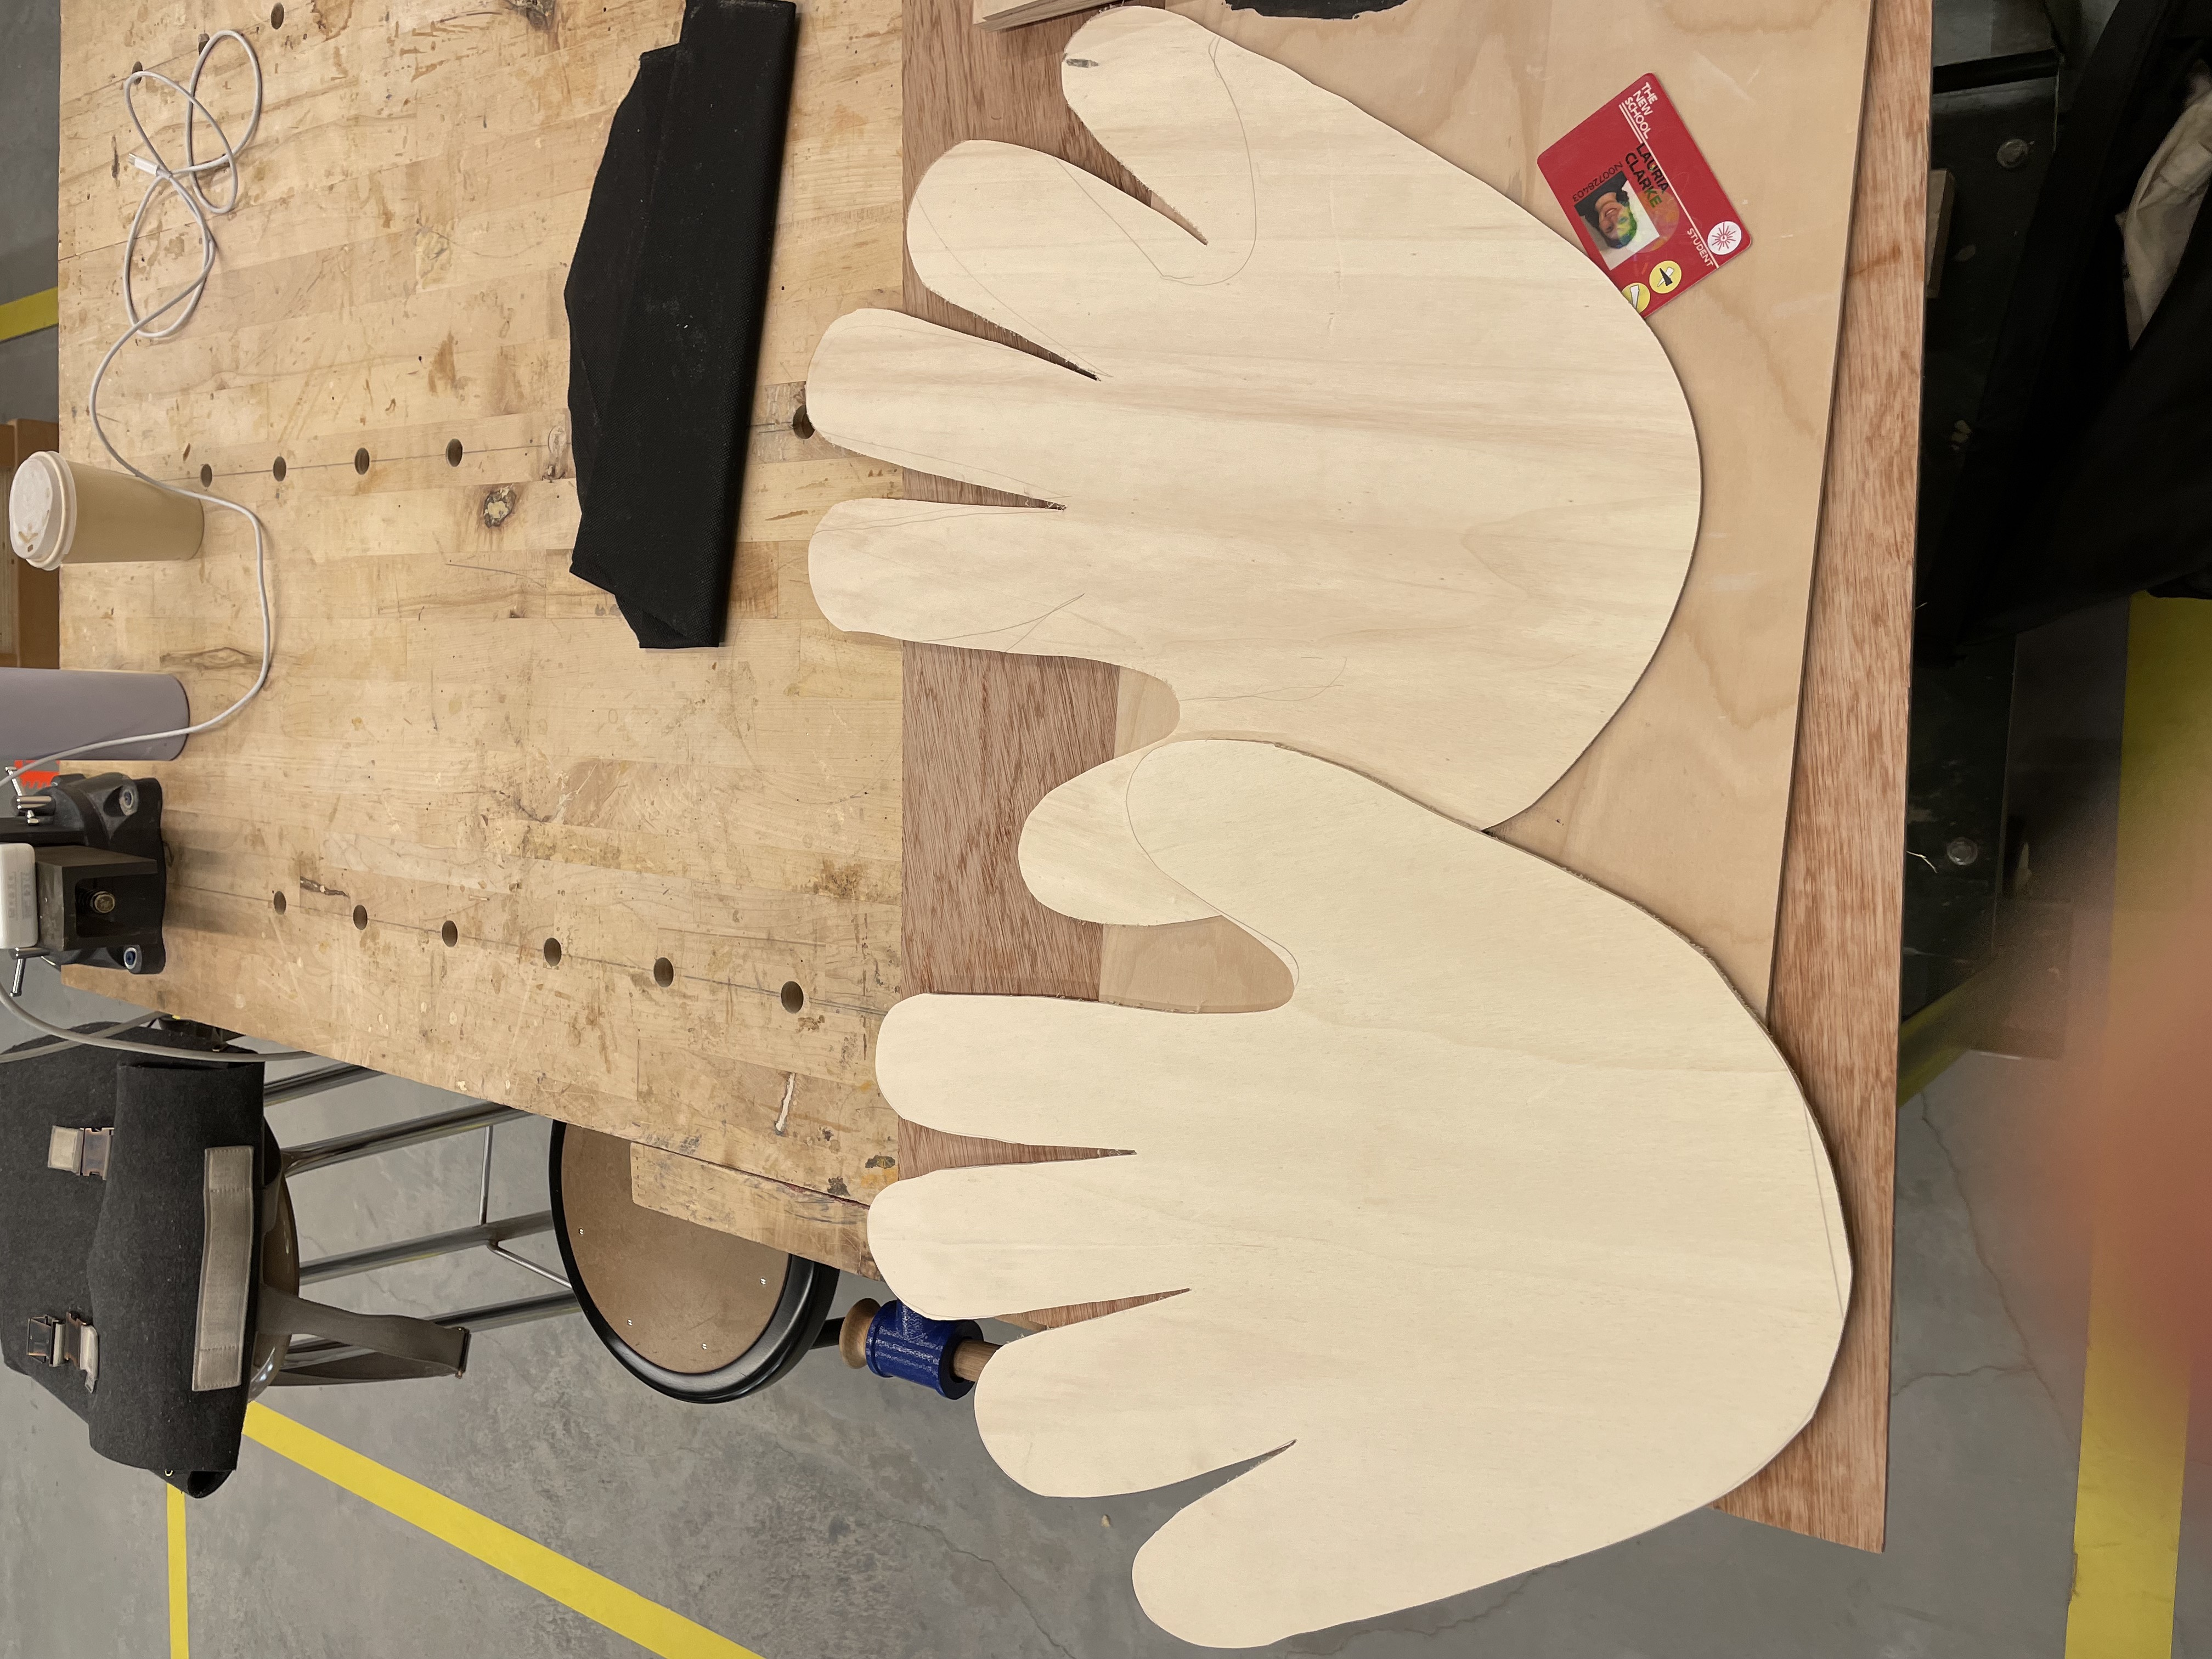
\includegraphics[width=0.5\textwidth, angle=270]{"images/III/plainhands.jpg"}
\caption{Big hands!}
\end{figure}

Next we found some $1/8$ inch and $3/4$ inch plywood and created the base of the new mechanism. At this point we also determined the best way to make the handle to activate the hand waving easier to use. A handle that needs to be pulled is a bit ambiguous and not very visual, so we decided to make the handle another lever in the shape of a hand that would encourage users to use their hands to activate it. This was a simple lever that sticks out of one side of the mechanism pulled one side of the hand waving lever down when activated. \href{https://drive.google.com/file/d/1A4jMRefTUcI-PZPhbS6XSqFU6V4kzS8j/view?usp=sharing}{Link to video of lever action.}  \href{https://drive.google.com/file/d/1zZMAdPojSRc_iC_QfIq4iEV6bjWMPP37/view?usp=sharing}{Link to video of the final lever mechanism.}

\begin{figure}[ht!]
\centering
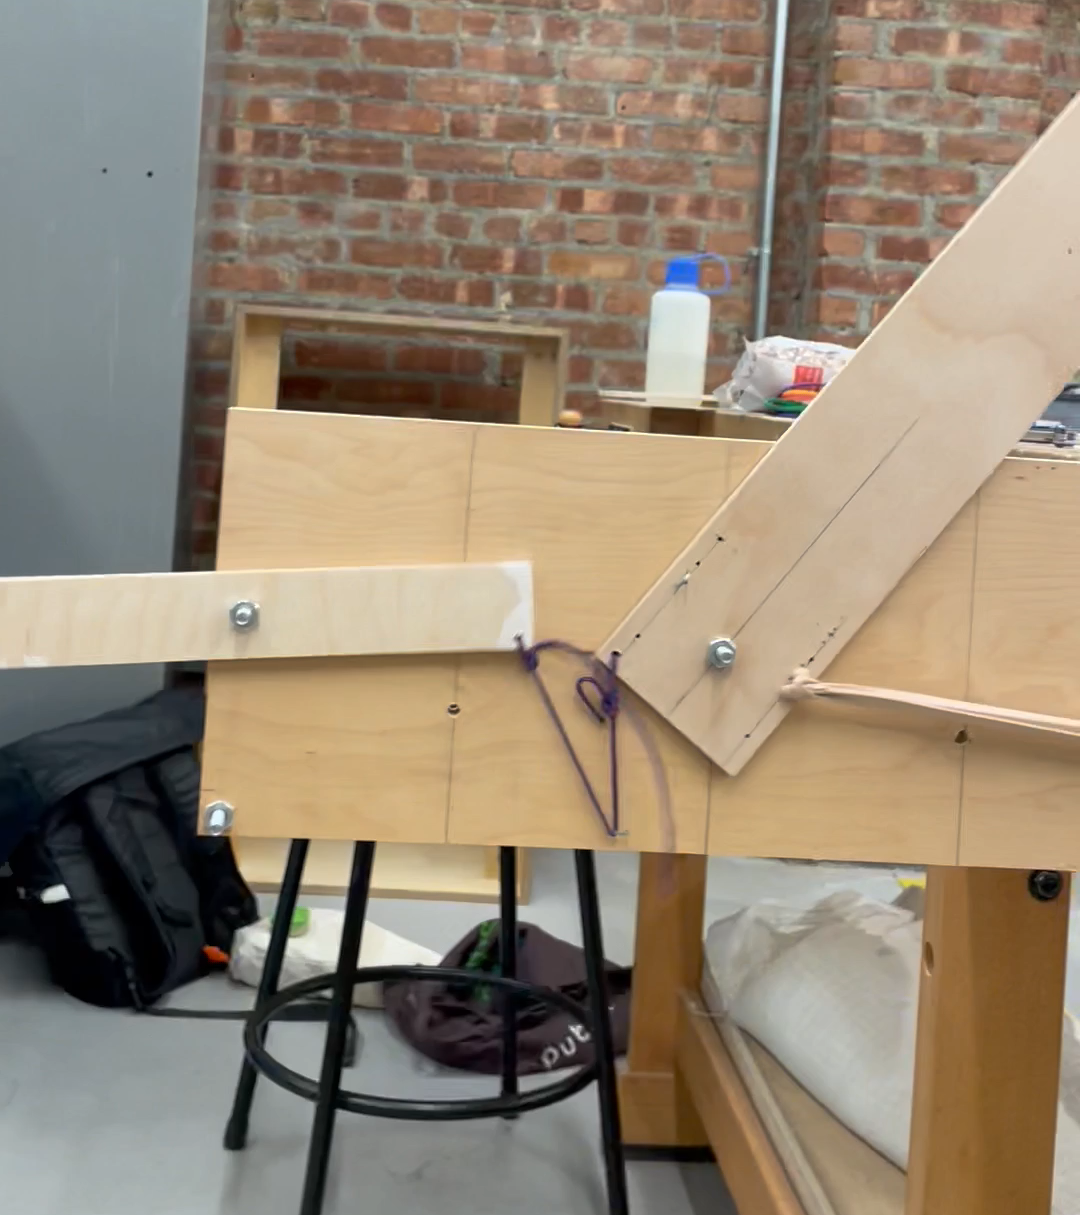
\includegraphics[width=0.6\textwidth]{"images/III/leverswithbase.png"}
\caption{Lever action.}
\end{figure}

Once the mechanism and base were dialed in, we painted the entire assembly using eye catching colors and a final layer of sparkly spray paint. The hope was that this would catch the light at night and make the hands more visible.

\begin{figure}[ht!]
\centering
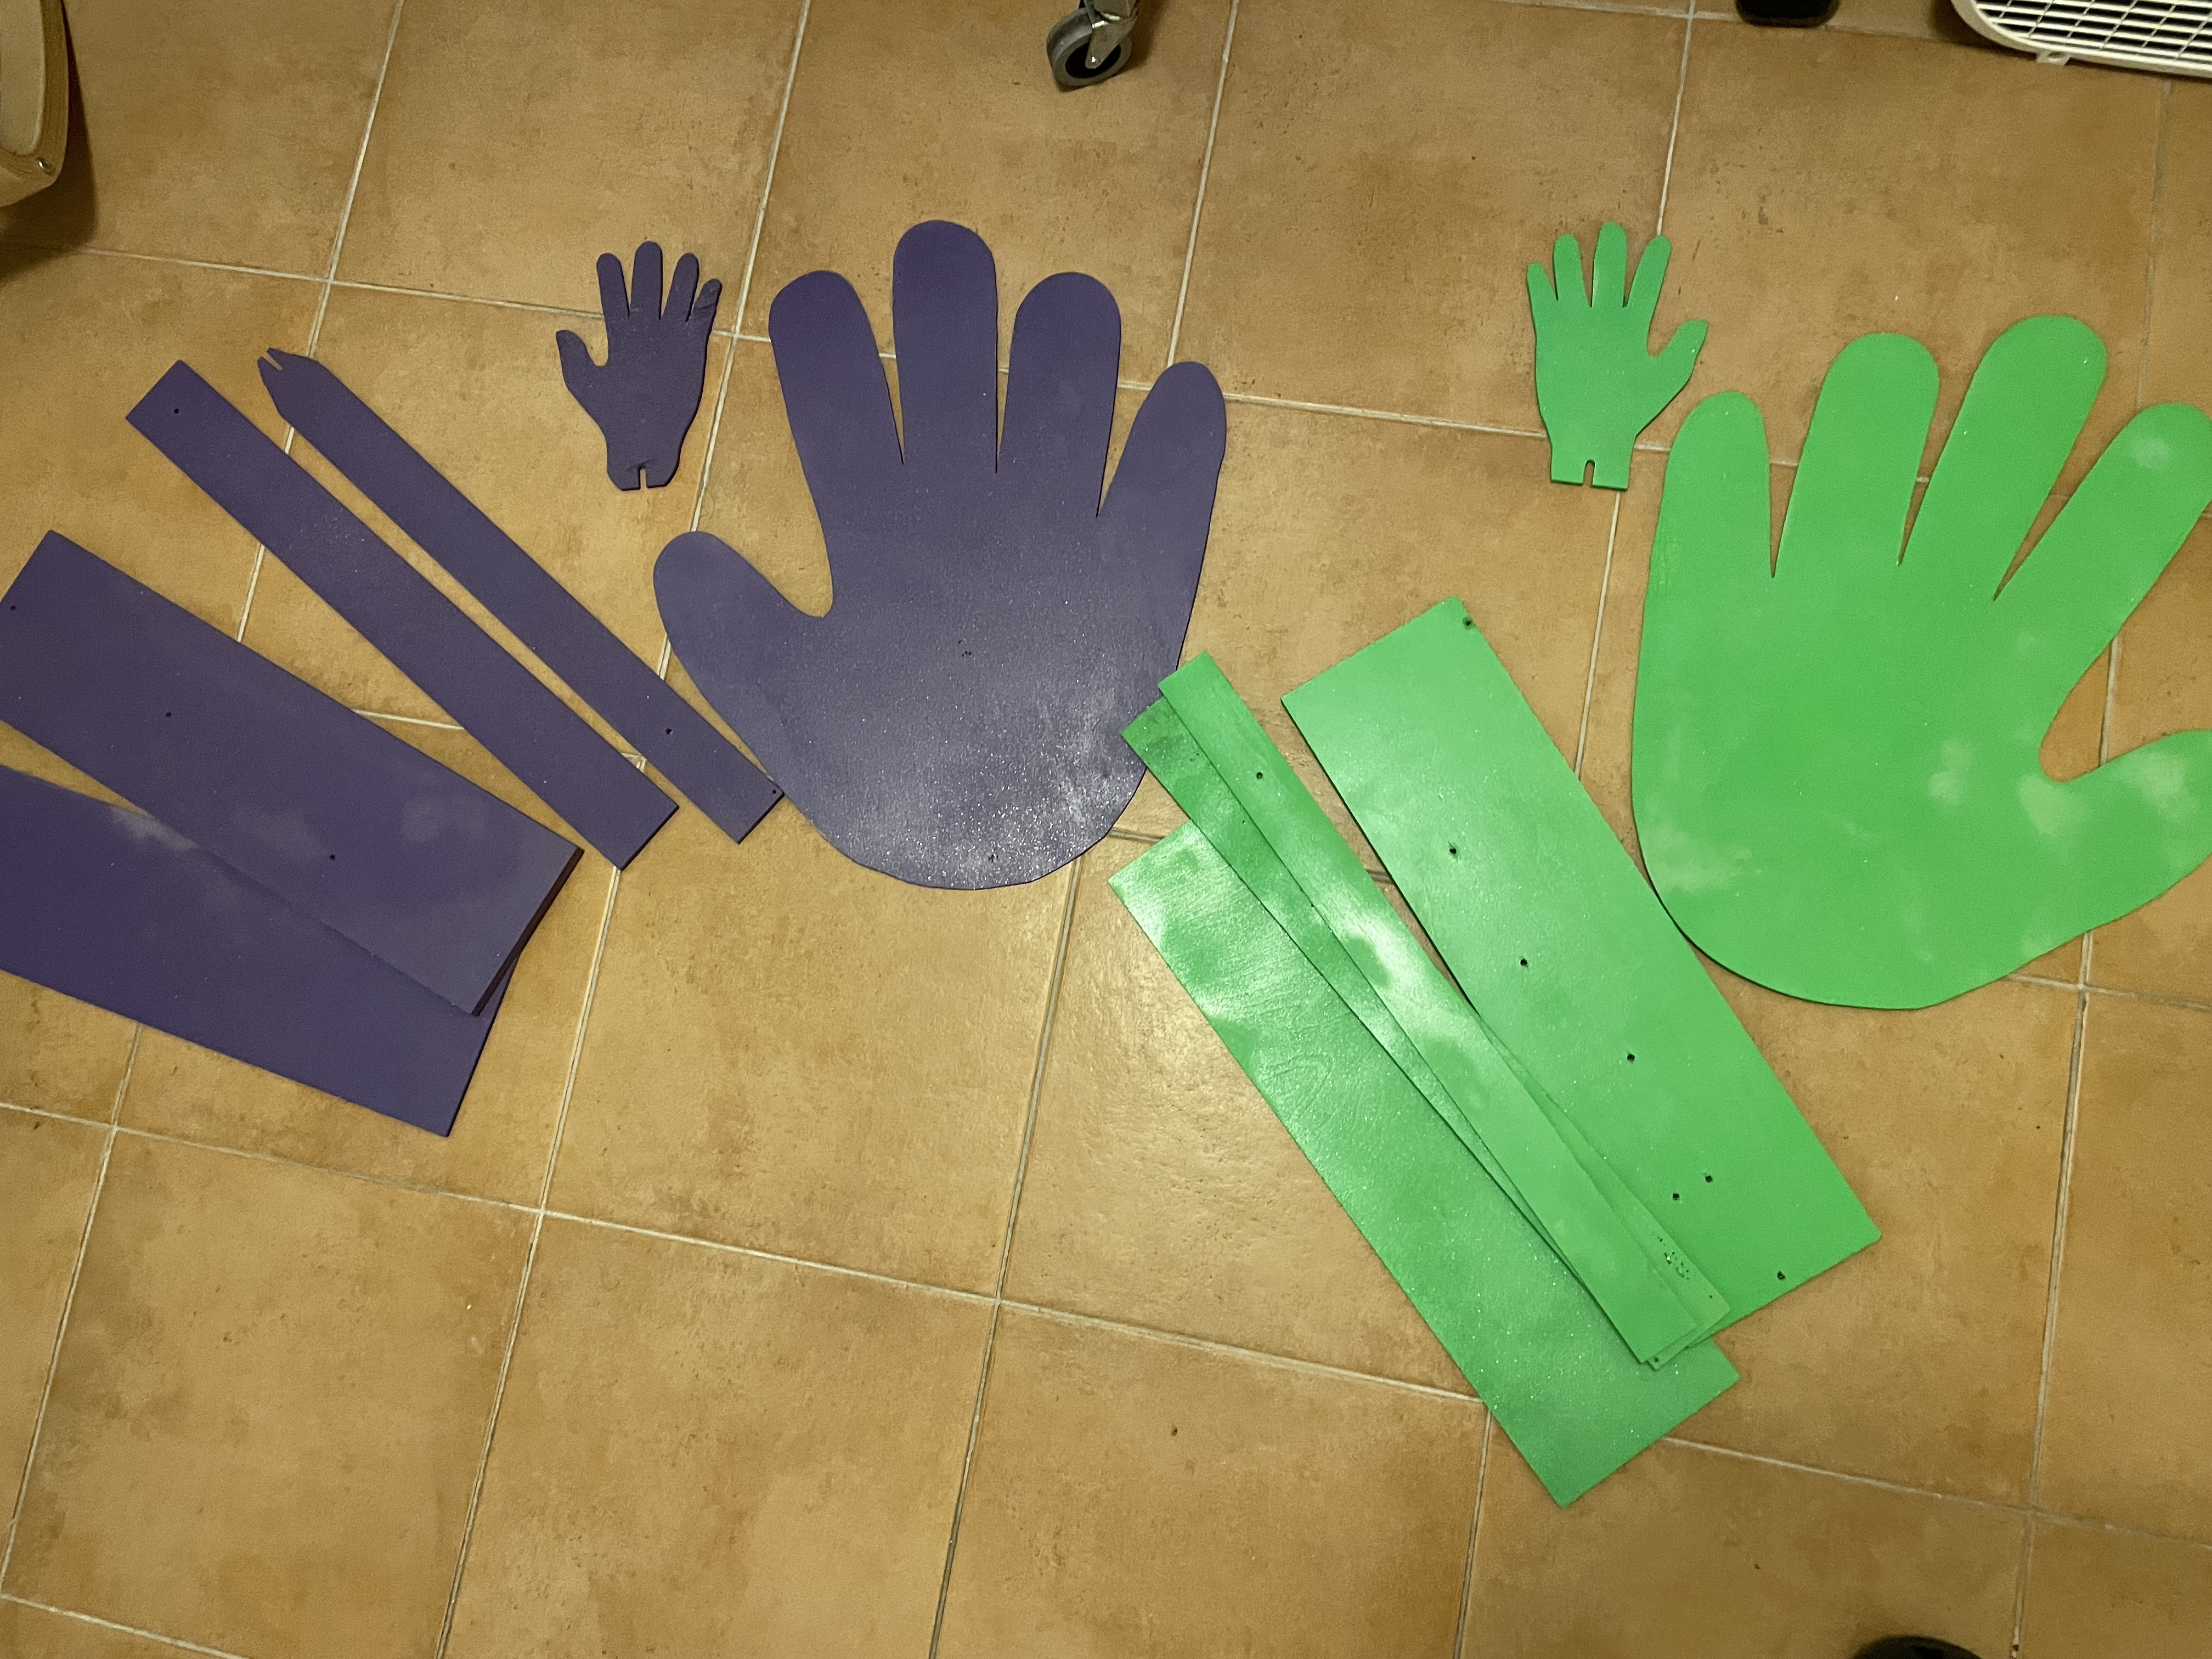
\includegraphics[width=0.5\textwidth]{"images/III/painting.JPG"}
\includegraphics[width=0.5\textwidth]{"images/III/elwire.JPG"}
\caption{Spray painted parts and installed EL wire.}
\end{figure}

We then added the electroluminescent wire around the perimeter of the large, waving hands and along the length of each lever to help attract more attention. Finally, after securing all the part in place, we were ready to install. 

\begin{figure}[ht!]
\centering
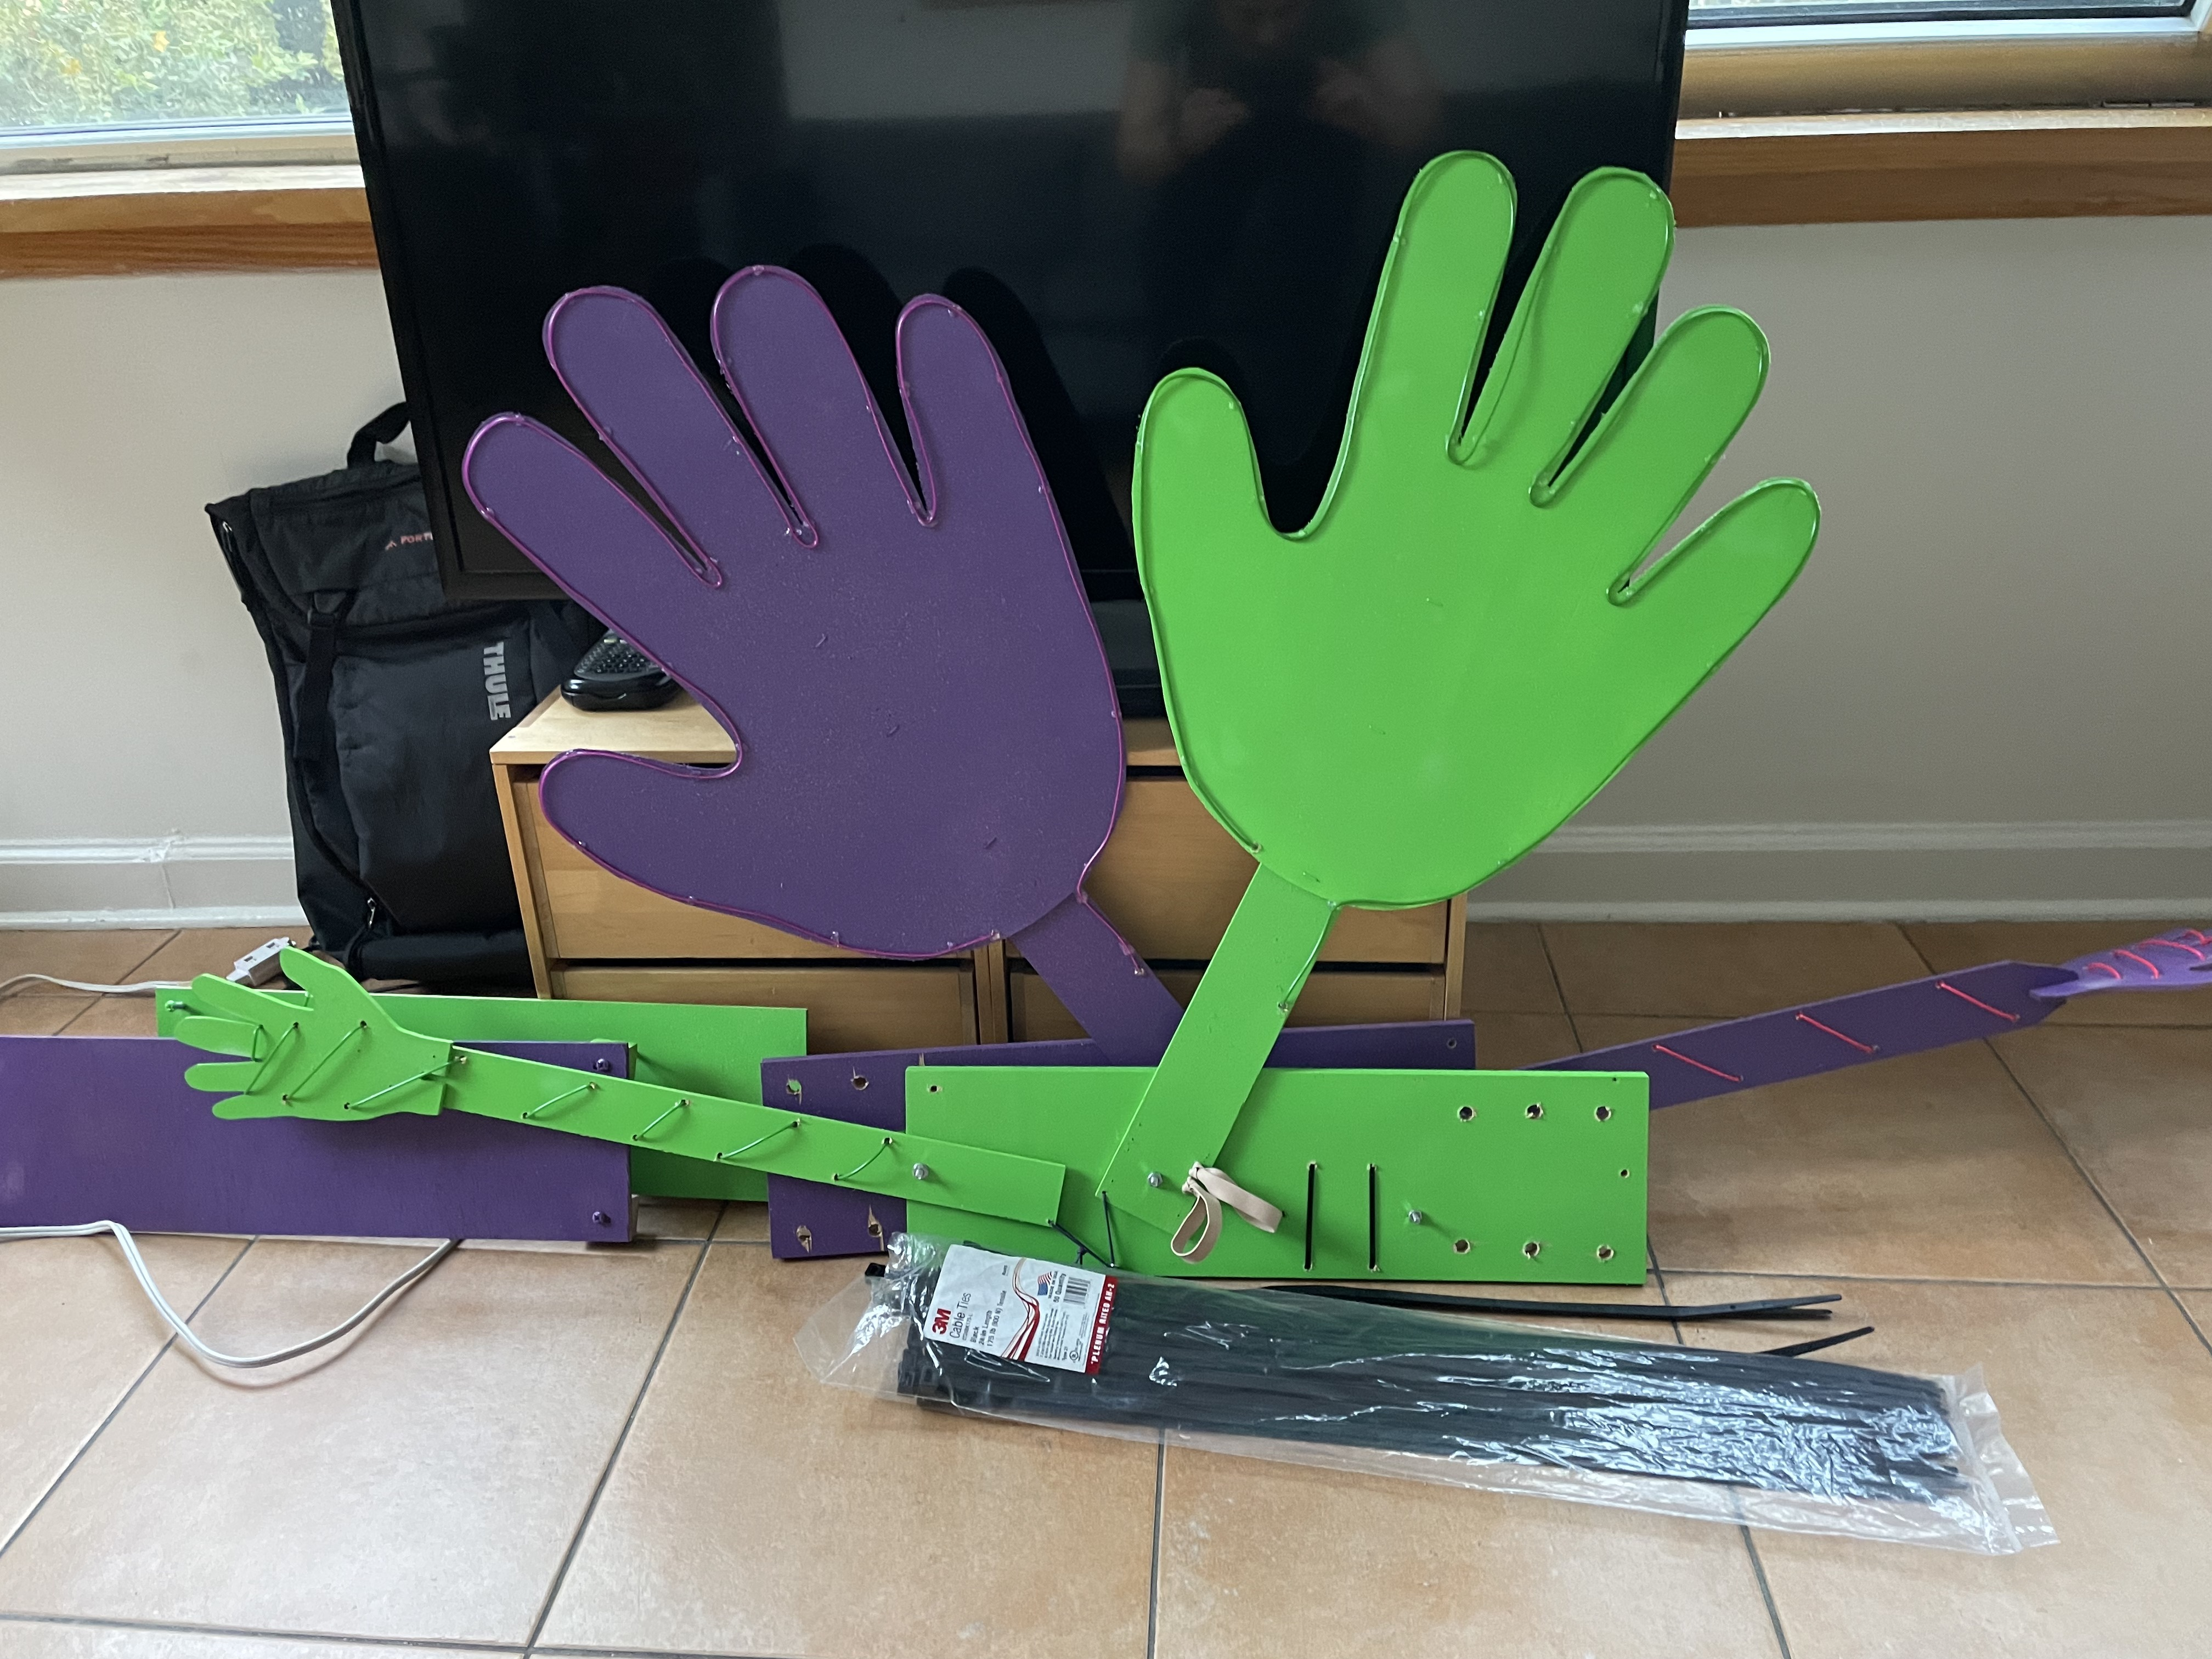
\includegraphics[width=0.5\textwidth]{"images/III/readytogo.JPG"}
\caption{Wave machine ready to install.}
\end{figure}



\clearpage
\section*{PART III - Installation}

Our installation too place in two parts. Once on the evening of September 17th and then again during later afternoon on September 26th. The first installation seems to generate more interest as it was later at night and the hands were more visible. During the second installation interest seems to increase as it became darker, however we were not able to stay and watch any later. 

Once we arrived at the first installation site, around 9PM, our plans had to be modified slightly. There was a large construction pylon on one side of the intended intersection making the space to walk in the crosswalk quite narrow. We were concerned that adding the wave machine to this side of the intersection would interfere too much with accessibility to the crosswalk, so we chose the perpendicular crosswalk at the intersection instead. This was an unfortunate change as the perpendicular intersection had a large pile of bagged trash next to it which decreased the amount of space around the hand installed there. Nevertheless, there was considerable interest almost as soon as we put up the hands.  

\begin{figure}[ht!]
\centering
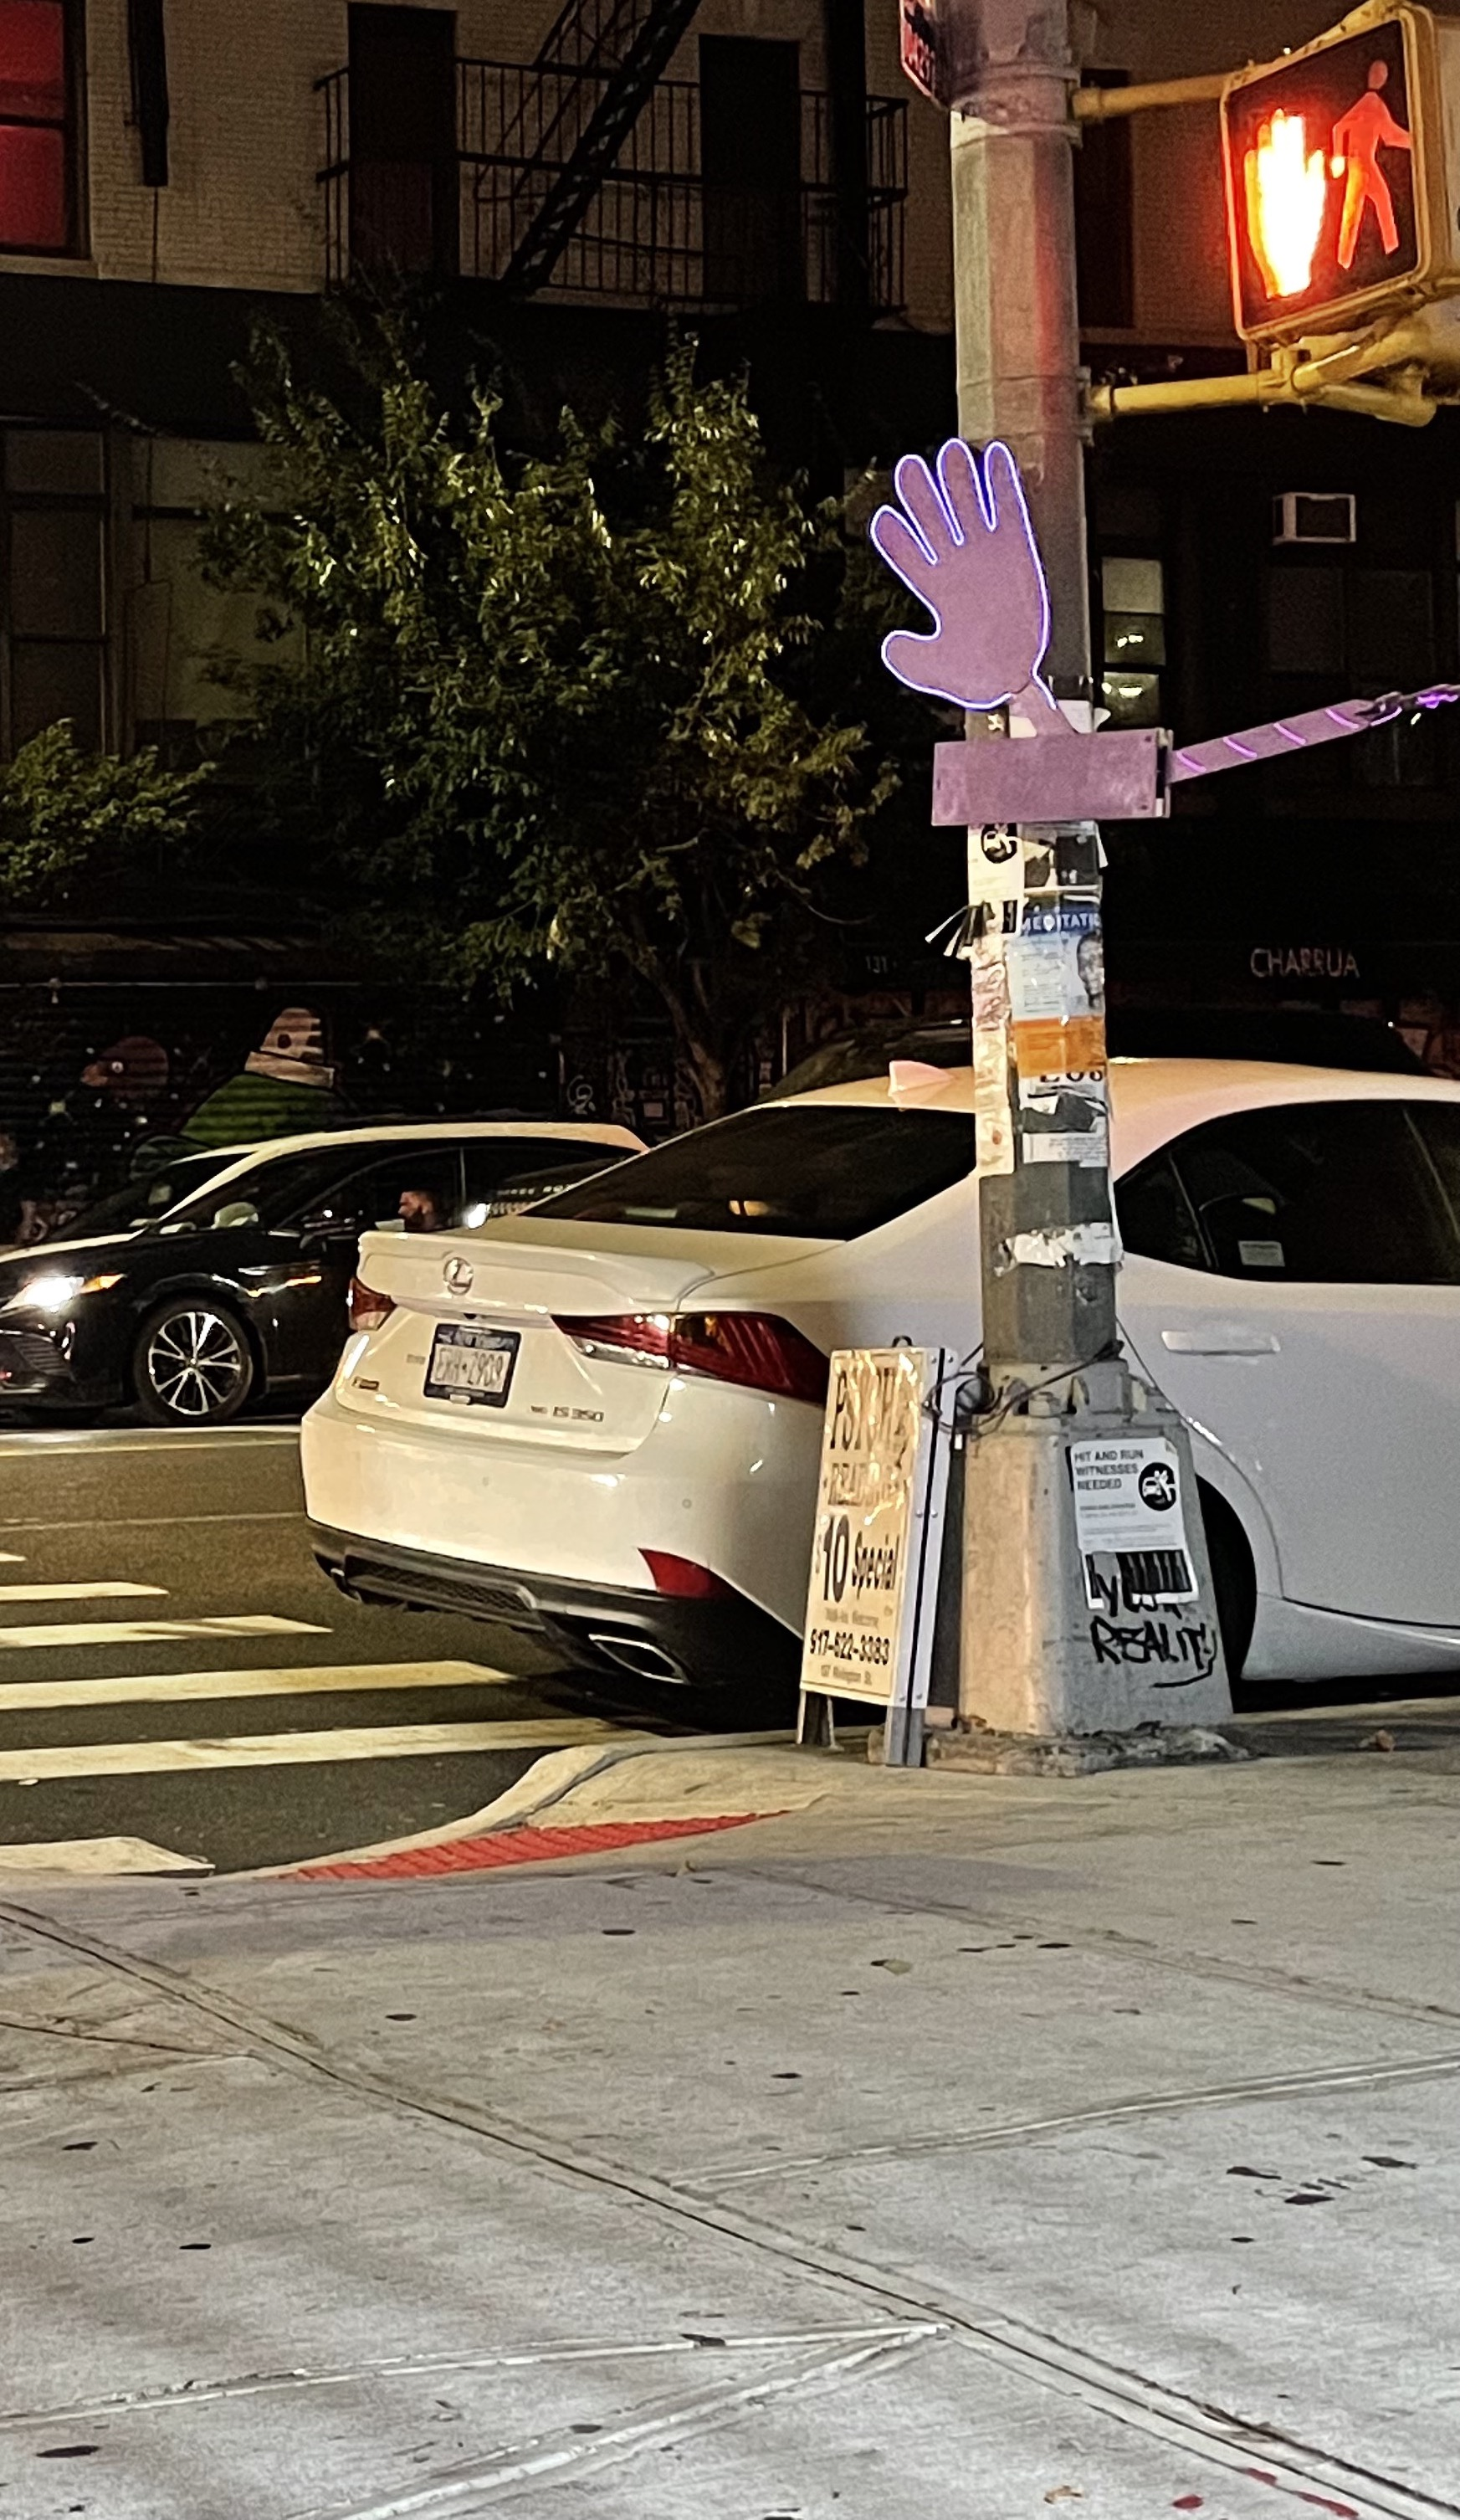
\includegraphics[width=0.45\textwidth]{"images/III/purplehandinstalled.JPG"}
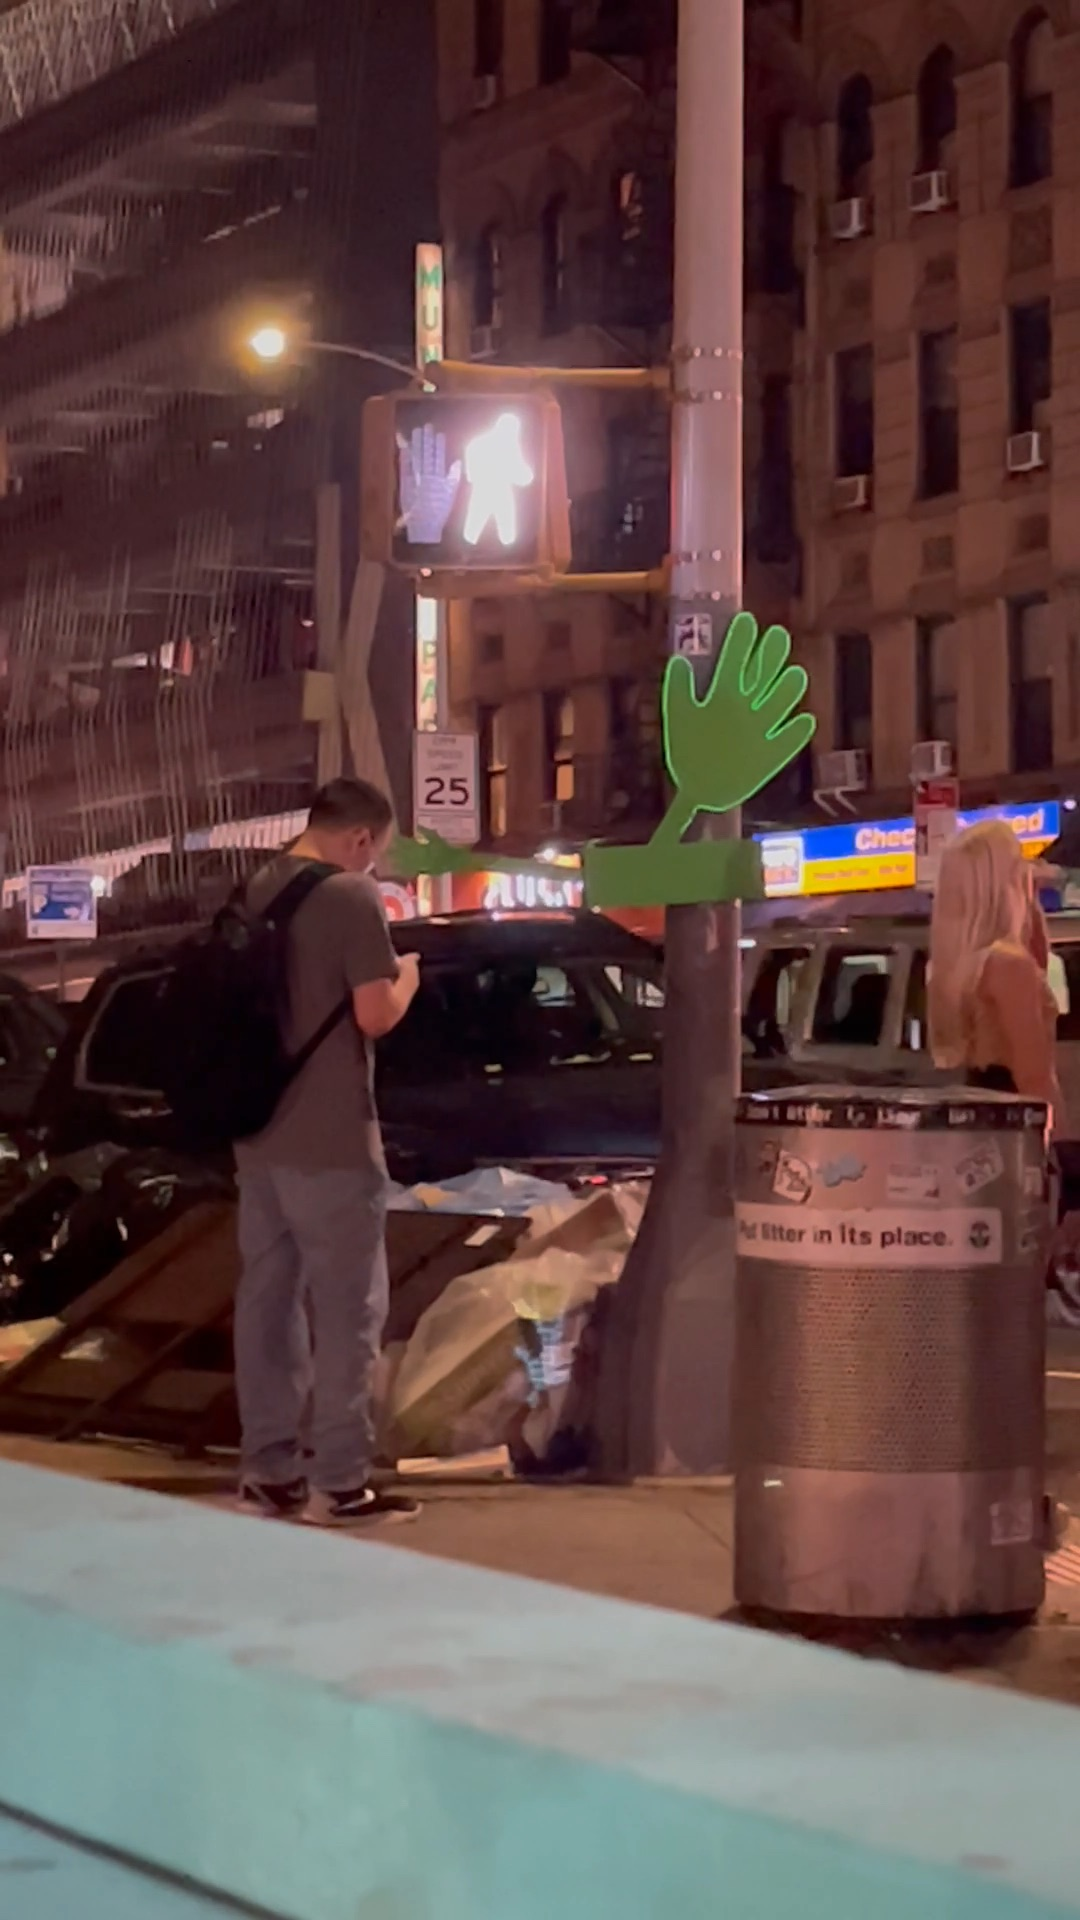
\includegraphics[width=0.45\textwidth]{"images/III/greenhandinstalled.JPG"}
  \caption{Hands installed on adjacent street corners around 9 PM (notice trash below green hand).}
\end{figure}

We chose to mount them high enough that they wouldn't be run into very often, but low enough that they were still visible to people on the street. During the second installation we tried lowering the hands on the street pole. Many more people ran into the lever and, while they were more visible, it wasn't entirely clear if this made it easier or harder to use them. 

Overall, the hands generated a lot of interest \href{https://drive.google.com/file/d/1pUGkjezofgZf2cuKnzpuoyqFLIYEEZ25/view?usp=sharing}{(see video of some "best of" interactions)}. The most challenging aspect of the installation process was waiting around long enough to observe good interactions. We would like to try installing the hands over a longer period of time and using a webcam to record all interactions. 

One thing that surprised us was how delicate people on the street treated the levers of the machine. Many people -- particularly during the second installation -- would come up to the hands and push lightly on the levers, not quite making them wave. For subsequent installations we plan to tune the mechanism so that it requires less force to achieve an exciting result. 

In conclusion, our interaction was quite effective! During the second installation we actually had a group of people wave at each other from across the street -- our intended result. By fine tuning the hands themselves, as well as our observation techniques, I think we can achieve more success in future installations. 



\end{document}
